% В этом документе преамбула

\documentclass[a4paper,12pt]{article}

\usepackage{lscape} % горизонтальный режим
\usepackage{pdflscape}

\usepackage{lipsum} % тестовые тексты

%%% Работа с русским языком
\usepackage{cmap}					% поиск в PDF
\usepackage{mathtext} 				% русские буквы в формулах
\usepackage[T2A]{fontenc}			% кодировка
\usepackage[utf8]{inputenc}			% кодировка исходного текста
\usepackage[english,russian]{babel}	% локализация и переносы
\usepackage{indentfirst}			% чтобы первый абзац в разделе отбивался красной строкой
\frenchspacing						% тонкая настройка пробелов
\usepackage{gensymb}				% символы по типу градусов
\usepackage{algorithm}				% для алгоритмов
\usepackage{algorithmic}			% для алгоритмов

%%% Приведение начертания букв и знаков к русской типографской традиции
\renewcommand{\epsilon}{\ensuremath{\varepsilon}}
\renewcommand{\phi}{\ensuremath{\varphi}}			% буквы "эпсилон"
\renewcommand{\kappa}{\ensuremath{\varkappa}}		% буквы "каппа"
\renewcommand{\le}{\ensuremath{\leqslant}}			% знак меньше или равно
\renewcommand{\leq}{\ensuremath{\leqslant}}			% знак меньше или равно
\renewcommand{\ge}{\ensuremath{\geqslant}}			% знак больше или равно
\renewcommand{\geq}{\ensuremath{\geqslant}}			% знак больше или равно
\renewcommand{\emptyset}{\varnothing}				% знак пустого множества

%%% Дополнительная работа с математикой
\usepackage{amsmath,amsfonts,amssymb,amsthm,mathtools,esint} % AMS
\usepackage{wasysym}
\usepackage{icomma} % "Умная" запятая: $0,2$ --- число, $0, 2$ --- перечисление

%% Номера формул
\mathtoolsset{showonlyrefs=true} % Показывать номера только у тех формул, на которые есть \eqref{} в тексте.

%% Свои команды

% операции, не определённые (или имеющие иные обохначения) в мат. пакетах
\DeclareMathOperator{\sgn}{\mathop{sgn}}				% ф-ия sgn
\renewcommand{\tg}{\mathop{\mathrm{tg}}\nolimits}		% обозначение тангенса

%% Перенос знаков в формулах (по Львовскому)
\newcommand*{\hm}[1]{#1\nobreak\discretionary{}
{\hbox{$\mathsurround=0pt #1$}}{}}

%%% Работа с картинками
\usepackage{graphicx}  				% Для вставки рисунков
\graphicspath{{images/}{images2/}}  % папки с картинками
\setlength\fboxsep{3pt} 			% Отступ рамки \fbox{} от рисунка
\setlength\fboxrule{1pt} 			% Толщина линий рамки \fbox{}
\usepackage{wrapfig} 				% Обтекание рисунков текстом

%%% Работа с таблицами
\usepackage{array,tabularx,tabulary,booktabs} 	% Дополнительная работа с таблицами
\usepackage{longtable}  						% Длинные таблицы
\usepackage{multirow}							% Слияние строк в таблице

%%% Теоремы

\newtheoremstyle{break}% name
	{}%         Space above, empty = `usual value'
	{}%         Space below
	{\itshape}% Body font
	{}%         Indent amount (empty = no indent, \parindent = para indent)
	{\bfseries}% Thm head font
	{.}%        Punctuation after thm head
	{\newline}% Space after thm head: \newline = linebreak
	{}%         Thm head spec
\theoremstyle{break}

% \theoremstyle{plain} % Стиль по умолчанию
\newtheorem{theorem}{Теорема}[section]
\newtheorem{lemma}{Лемма}[section]
\newtheorem{definition}[theorem]{Определение}
\newtheorem{property}{Свойство}
 
\newtheorem{corollary}{Следствие}[theorem]

\newtheoremstyle{example}	% style name
	{2ex}					% above space
	{2ex}					% below space
	{}						% body font
	{}						% indent amount
	{\bf}				% head font
	{.}						% post head punctuation
	{\newline}				% post head punctuation
	{\thmname{#1}\thmnumber{ #2}\thmnote{ (#3)}}						% head spec

\theoremstyle{example}
\newtheorem{exmp}{Пример}[section]
 
\theoremstyle{remark} % "Примечание"
\newtheorem*{nonum}{Решение}
\newtheorem*{evidence}{Доказательство}
\newtheorem*{remark}{Примечание}

%%% Программирование
\usepackage{etoolbox} % логические операторы

%%% Страница
\usepackage{extsizes} % Возможность сделать 14-й шрифт
\usepackage{geometry} % Простой способ задавать поля
	\geometry{top=15mm}
	\geometry{bottom=35mm}
	\geometry{left=10mm}
	\geometry{right=10mm}

%\usepackage{fancyhdr} % Колонтитулы
% 	\pagestyle{fancy}
 	%\renewcommand{\headrulewidth}{0pt}  % Толщина линейки, отчеркивающей верхний колонтитул
% 	\lfoot{Нижний левый}
% 	\rfoot{Нижний правый}
% 	\rhead{Верхний правый}
% 	\chead{Верхний в центре}
% 	\lhead{Верхний левый}
%	\cfoot{Нижний в центре} % По умолчанию здесь номер страницы

\usepackage{setspace} % Интерлиньяж (межстрочные интервалы)
%\onehalfspacing % Интерлиньяж 1.5
%\doublespacing % Интерлиньяж 2
%\singlespacing % Интерлиньяж 1

\usepackage{lastpage} % Узнать, сколько всего страниц в документе.

\usepackage{soulutf8} % Модификаторы начертания

\usepackage{hyperref}
\usepackage[usenames,dvipsnames,svgnames,table,rgb]{xcolor}
\hypersetup{				% Гиперссылки
    unicode=true,           % русские буквы в раздела PDF
    pdftitle={Заголовок},   % Заголовок
    pdfauthor={Автор},      % Автор
    pdfsubject={Тема},      % Тема
    pdfcreator={Создатель}, % Создатель
    pdfproducer={Производитель}, % Производитель
    pdfkeywords={keyword1} {key2} {key3}, % Ключевые слова
    colorlinks=true,       	% false: ссылки в рамках; true: цветные ссылки
    linkcolor=MidnightBlue, % внутренние ссылки
    citecolor=black,        % на библиографию
    filecolor=magenta,      % на файлы
    urlcolor=blue           % на URL
}

\usepackage{csquotes} % Еще инструменты для ссылок

%\usepackage[style=authoryear,maxcitenames=2,backend=biber,sorting=nty]{biblatex}

\usepackage{multicol} % Несколько колонок

%%% Работа с графикой
\usepackage{tikz}
\usetikzlibrary{calc}
\usepackage{tkz-euclide}
\usetikzlibrary{arrows}
\usepackage{pgfplots}
\usepackage{pgfplotstable}

%%% Настройка подписей к плавающим объектам
% \usepackage{floatrow}	% размещение
\usepackage{caption}	% начертание
\captionsetup[figure]{labelfont=bf,textfont=it,font=footnotesize}	% нумерация и надпись курсивом
% для подфигур: заголовок подписи полужирный, текст заголовка обычный
% выравнивание является неровным (т.е. выровненным по левому краю)
% singlelinecheck = off означает, что настройка выравнивания используется, даже если заголовок имеет длину только одну строку.
% если singlelinecheck = on, то заголовок всегда центрируется, когда заголовок состоит только из одной строки.
\captionsetup[subfigure]{labelfont=bf,textfont=normalfont,singlelinecheck=off,justification=raggedright}

%%% Stuff для листинга
\usepackage{listings}
\usepackage{xcolor}

\colorlet{mygray}{black!30}
\colorlet{mygreen}{green!60!blue}
\colorlet{mymauve}{red!60!blue}

\lstset{
	backgroundcolor=\color{gray!10},  
	basicstyle=\ttfamily,
	columns=fullflexible,
	breakatwhitespace=false,      
	breaklines=true,                
	captionpos=b,                    
	commentstyle=\color{mygreen}, 
	extendedchars=true,              
	frame=single,                   
	keepspaces=true,             
	keywordstyle=\color{blue},      
	language=c++,                 
	numbers=none,                
	numbersep=5pt,                   
	numberstyle=\tiny\color{blue}, 
	rulecolor=\color{mygray},        
	showspaces=false,               
	showtabs=false,                 
	stepnumber=5,                  
	stringstyle=\color{mymauve},    
	tabsize=3,                      
	title=\lstname                
}

% для извращённых начертаний
\usepackage{mathrsfs}

\usepackage{makecell}
\setcellgapes{3pt}

% Зачёркивание символов
\usepackage{cancel}

% перечисления с буквами
\usepackage{enumitem}

\begin{document}
	
\renewcommand{\figurename}{Рисунок}

\tableofcontents

\newpage

\section{Свойства вероятности.}

Отталкиваемся от общей модели: пусть $(\Omega, \mathcal{F}, P)$ - вероятностный эксперимент. $A, B \in \mathcal{F}$.

\begin{enumerate}
	\item $P(\emptyset) = 0$
	\item Если определено событие $A$, то определено и обратное ему $\bar A = \Omega \backslash A$ такое, что $P(A) + P( \bar A) = 1$.
	\item $B \supseteq A \Rightarrow P(B \backslash A) = P(B) - P(A)$. 
	
	\noindent 3.' (Монотонность) $A \subset B$ (в этом случае принято говорить, что "событие $A$ предшествует событию $B$"\, или "событие $A$ влечёт за собой событие $B$"\,) $\Rightarrow P(B) \ge P(A)$. Это следует из того, что $P(A) + P(\bar A B) = P(B)$.
	
	\item $A, B \in \mathcal{F} \Rightarrow P(A \cup B) = P(A) + P(B) - P(AB) $. 
	
	\noindent 4.' $-//- \Rightarrow P(A \cup B) \le P(A) + P(B)$
	
	\item Формула включения исключения: 
	\[A_1, \dots, A_n \in \mathcal{F}: \]
	\[P \left(\bigcup_{i=1}^{n} A_i \right) = \sum_{s=1}^{n} \sum_{|\sigma| = s} (-1)^{s-1} P \left(\bigcap_{i \in \sigma} A_i \right) = \] 
	\[= P(A_1) + \dots + P(A_n) - P(A_1 A_2) - P(A_1 A_3) - \dots \pm (-1)^n P(A_1, \dots, A_n) \]
	
	\noindent $\sigma$ - сочетание индексов $\{ 1, \dots, n \}, s = |\sigma|$ - число элементов сочетания.
	\item Свойство непрерывности ($\eq$ АВ1, АВ3):
	
	$\letus$ имеется вложенный $\infty$ набор "расширяющихся"\, событий: $ A_1 \subset A_2 \subset \dots A_i \in \mathcal{F} $, тогда
	\[ \lim_{n \to \infty} P \left( \bigcup_{i=1}^{n} A_i \right) = P \left( \bigcup_{i=1}^{\infty} A_i \right) = \lim_{n \to \infty} P(A_n) \]
	
	\noindent 6.' (Комплементарное свойство) $A_1 \supset A_2 \supset \dots A_i \in \mathcal{F}$
	\[ \lim_{n \to \infty} P \left( \bigcap_{i=1}^{n} A_i \right) = \lim_{n \to \infty} P(A_1) \]
\end{enumerate}

\section{В каком случае события $A_1 \dots A_n$ называются независимыми в совокупности?}

$\letus (\Omega, \mathcal{F}, P)$ - вероятностный эксперимент.

События $A_1, \dots, A_n \in \mathcal{F}$ называются независимыми в совокупности (взаимно независимыми), если для $\forall \{ i_1, \dots, i_s \} \subseteq \{ 1, \dots, n \}, s \in [1, n]$ ($\eq$ любого сочетания индексов) верно:
\[ P(A_{i_1} \dots A_{i_s}) = P(A_{i_1}) \cdot ... \cdot P(A_{i_s}), s = 1, \dots, s \]

Несколько событий называются независимыми в совокупности (или просто независимыми), если независимы каждые два из них и независимы каждое из них и все возможные произведения остальных.

\section{Формула полной вероятности.}

Пусть $\{A_i\}_{i=1}^{n}$ - ПГС и для всех $i \ge 0$ верно нер-во $P(A_i) > 0$. Тогда для любого случайного события $B$ его вероятность можно вычислить по формуле:
\[ P(B) = \sum_{i} P(B|A_i) P(A_i) \]

\begin{remark}
	Количество элементов полной группы событий может быть и бесконечным, но обязательно счетным.
\end{remark}

\noindent \textbf{Для абсолютно непрерывных величин:}

Пусть $\xi_1, \xi_2$ - абсолютно непрерывные случайные величины на $(\Omega, \mathcal{F}, P)$ с совместной плотностью распределения $p_{\vec{\xi}}(x,y)$.

\[\eta=\xi_1+\xi_2\]
\[p_\eta(t)=\int_\mathbb{R} p_{\xi_1|\xi_2=y} (t-y) p_{\xi_2} (y)dy = \int_\mathbb{R} p_{\xi_2|\xi_1=x}(t-x) p_{\xi_1}(x)dx\]

\noindent Если $\xi_1, \xi_2$ - независимы, то
\[ p_{\vec{\xi}} (x, y) = p_{\xi_1} (x) p_{\xi_2} (y); ~~~~~~~~~ p_{\xi_1 | \xi_2} = y(x) = p_{\xi_1} (x) \]

\noindent Отсюда можно получить формулу свёртки для плотностей:
\[ p_{\eta} (t) = \int_{\mathbb{R}} p_{\xi_1} (t - y) p_{\xi_2} (y) dy = \int_{\mathbb{R}} p_{\xi_2} (t - x) p_{\xi_1} (x) dx \]

\noindent Можно использовать и для других функций, например, $\eta = \xi_1 \xi_2$:
\[ p_{\eta} (t) = \int_{\mathbb{R}} p_{\xi_1 | \xi_2 = y} \left( \frac{t}{y} \right) p_{\xi_2} (y) dy \]

\noindent \textbf{Что такое ПГС?}

Пусть $ \{ H_i \}_{i=1}^n $ - некоторый набор случайных событий. Назовём его ПГС, если выполняются следующие условия:
\begin{enumerate}
	\item $H_i \cap H_j = \emptyset$ - события попарно несовместны (не могут появится одновременно в рез-те однократного проведения эксперимента).
	\item $\bigcup\limits_{i=1}^{n} H_i = \Omega$
	\item $P(H_i) > 0, \forall i$
\end{enumerate}

\begin{remark}
	Независимость $\Rightarrow (\cancel{\Leftarrow})$ попарная независимость.
\end{remark}

\section{Формулы Байеса.}

По формуле Байеса можно более точно пересчитать вероятность, беря в расчет как ранее известную информацию, так и данные новых наблюдений. Формула Байеса позволяет «переставить причину и следствие»: по известному факту события вычислить вероятность того, что оно было вызвано данной причиной. События, отражающие действие «причин», в данном случае называют гипотезами, так как они — предполагаемые события, повлекшие данное.

~

Дадим математическую формулировку:

\noindent $\letus A \in \mathcal{F} (P(A) > 0), \{ H_i \}_{i=1}^n$ - ПГС и для всех $i \ge 1$ верно неравенство $P(H_i) > 0$. Тогда
\[ P(H_i|A) = \frac{P(A|H_i) \cdot P(H_i)}{\sum\limits_{j=1}^{n} P(A|H_j) \cdot P(H_j)} \]

Объяснения:
\begin{itemize}
	\item $\sum\limits_{j=1}^{n} P(A|H_j) \cdot P(H_j)$ - вероятность $A$, разложенная по ф-ле полной вероятности.
	\item $P(H_i)$ - априорные (судим о результатах до проведения эксперимента).
\end{itemize}

\begin{proof}
	\[ \frac{P(A|H_i)P(H_i)}{\sum\limits_{j \ge 1} P(A|H_j)P(H_j)} = \frac{P(A|H_i) P(H_i)}{P(A)} = \frac{P(H_iA)\cancel{P(H_i)}}{\cancel{P(H_i)}P(A)} = P(H_i|A) \]
\end{proof}

\begin{figure}[h]
	\center{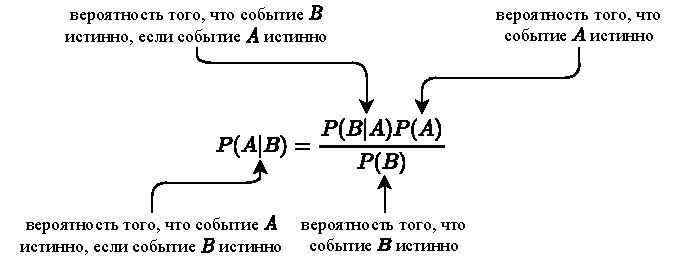
\includegraphics[scale=0.9]{./media/3.5.pdf}}
\end{figure}

\begin{remark}
	Формула работает, когда есть несколько последовательных событий и последующее считать легче, что какое-то 1-ое уже произошло.
\end{remark}

\section{Что такое испытания Бернулли и Формула Бернулли?}

\textbf{Испытание} - эксперимент с 2-мя исходами
\[ \Omega = \{\text{'успех'}, \text{'неудача'}\} ~~~~~~~~~~~ \mathcal{F} - \text{все п/н } \Omega \]
\[ P(\{\text{'у'}\}) = 1 - P(\{\text{'н'}\}) = p, p \in [0,1] \]

\textbf{Испытание Бернулли} - это совокупность $n$ независимых испытаний с одинаковой вероятностью успеха $P(\{\text{'у'}\}) = p, p \in [0,1]$.

\noindent Исход $\omega = (i_1, \dots, i_n), i_j \in \{\text{'у', 'н'}\}$

\noindent $\# \Omega = 2^n$, где $n$ - число испытаний Бернулли.

\noindent $P(\{\omega\}) = p^k(1-p)^{n-k}, k - $ число 'у' в последовательности ($i_1, \dots, i_n$).

В $n$ испытаниях Бернулли изучают:
\begin{enumerate}
	\item $\mu_n$ - число успехов в $n$ испытаниях Бернулли.
	\item $\nu_1$ - число успехов до 1-ой неудачи.
	\item $\nu_k$ - число успехов до $k$-ой неудачи.
\end{enumerate}

\textbf{Формула Бернулли.}

\[ P(\mu_n = k) = C_n^kp^k(1-p)^{n-k} = C_n^k p^k q^{n-k}, k = 0,1, \dots, n \]

\section{Интегральная теорема Муавра-Лапласа.}

Пусть $\xi_1, \xi_2, \dots$ - последовательность независимых одинаково распределенных случайных величин, с распределением Бернулли, то есть $P(\xi_k = 1) = 1 - P(\xi_k = 0) = p$, где $0 < p < 1$.

Каждую из случайных величин $\xi_k$ можем интерпретировать как результат при $k$-ом испытании. Если случайная величина приняла значение $1$, то это означает, что в $k$-ом испытании произошел «успех», если $\xi_k$ приняла значение 0, то в $k$-ом испытании - «неудача». Тогда $\mu_n = \sum\limits_{k=1}^{n} \xi_k$ означает число «успехов» в $n$ испытаниях. Для этих случайных величин $E\xi_k = p, D\xi_k = p(1-p)$. Тогда выполнены условия теоремы Леви, и, следовательно, выполняется соотношение из ЦПТ Леви для всех $x \in \mathbb{R}$.

\[ \underset{-\infty \le a < b \le \infty}{sup} \left| P_n \left( a \le \dfrac{\mu_n - np}{\sqrt{np(1 - p)}} < b \right) - \int_{a}^{b} \dfrac{1}{\sqrt{2 \pi}} e^{-\frac{t^2}{2}}dt \right| \underset{n \to \infty}{\to} 0 \]

Если учесть монотонность и поведение на бесконечностях функций распределения, что приводит к окончательному выводу, фиксирующему наличие равномерной сходимости:

Всё аналогично, только вместо интеграла записываем $- (\Phi (b) - \Phi (a))$.

\noindent \textbf{Следствие:}

Если устремим $a$ к минус бесконечности, а $b$ к бесконечности, то получим равенство
\[ \frac{1}{\sqrt{2 \pi}} \int_{-\infty}^{\infty} e^{-\frac{t^2}{2}} dt = 1 \]

\noindent \textbf{Как применять данную теорему?} Если $n$ очень большое, то
\[ P(\alpha \le k \le \beta) = P \left( \frac{\alpha - np}{\sqrt{npq}} \le \frac{k - np}{\sqrt{npq}} < \frac{\beta - np}{\sqrt{npq}} \right) \approx \]
\[ \approx \frac{1}{\sqrt{2 \pi}} \int\limits_{\frac{\alpha - np}{\sqrt{npq}}}^{\frac{\beta - np}{\sqrt{npq}}} e^{-\frac{t^2}{2}} dt = \Phi \left( \frac{\beta - np}{\sqrt{npq}} \right) - \Phi \left( \frac{\alpha - np}{\sqrt{npq}} \right), \]
где функция $\Phi (x)$ определяется следующим равенством:
\[ \Phi (x) = \frac{1}{\sqrt{2 \pi}} \int_{-\infty}^{x} e^{-\frac{t^2}{2}} dt = \int_{-\infty}^{x} \phi (t) dt \]

\section{Теорема Пуассона и как её применять.}

\noindent \textbf{Схема Пуассона}

Рассматривают последовательность серий испытаний Бернулли, где $n$ испытаний, при этом $n \to \infty$, но $\lambda = n p_n = const$. $P(\mu_n = k), k$ - не меняется с ростом $n$.
\[ p = p_n = \dfrac{\lambda}{n}, \lambda > 0 \]

\noindent \textbf{Теорема Пуассона}

В схеме Пуассона при фиксированном $k \in 0,1, \dots$

\[ \left| P(\mu_n = k) - \dfrac{\lambda^k}{k!}e^{-\lambda} \right| \underset{n \to \infty}{\to} 0 ~~~~~~~~~~~~~~ \left( P(\mu_n = k)\underset{n \to \infty}{\to} \dfrac{\lambda^k}{k!}e^{- \lambda} \right) \]

\noindent \textbf{Формула Пуассона}

\[ P(\mu_n = k) \approx \dfrac{\lambda^k}{k!}e^{-\lambda} \]

\begin{remark}
	При большой величине $np$ - МЛ, при малом - Пуассон.
	
	Обычно границу ставят: $np \ge 10$ и $np < 10$.
\end{remark}

\section{Локальная теорема Муавра-Лапласа.}

Рассмотрим $n$ испытаний Бернулли, где $p = P(\text{'у'})$ - вероятность успеха в одном испытании, $k$ - число успехов в $n$ испытаниях. Введем следующие обозначение $x_{n, k} = \frac{k - np}{\sqrt{npq}}, q = 1 - p$.

Справедливо следующее соотношение
\[ \dfrac{P_n(k)}{\frac{1}{\sqrt{npq}} \cdot \frac{1}{\sqrt{2 \pi}} \cdot e^{- \frac{(x_{n, k})^2}{2}}} \to 1 ~~~~~~ (n \to \infty) \]
равномерно по всем таким $k$, для которых при произвольных фиксированных $c > 0$ и $\epsilon > 0$ выполнено неравенство: $|x_{n, k}| \le c \cdot n^{\frac{1}{6} - \epsilon}$.

Утверждение теоремы означает, что
\[ P_n(k) \approx \frac{1}{\sqrt{npq}} \cdot \frac{1}{\sqrt{2 \pi}} e^{-\frac{x_{n,k}^2}{2}} = \frac{1}{\sqrt{npq}} \phi (x_{n, k}), \]
где $\phi(x) = \frac{1}{\sqrt{2 \pi}} e^{- \frac{x^2}{2}}$ - \textit{функция Гаусса}.

\section{Аксиомы вероятности.}

Аксиоматика Колмогорова - общепринятая аксиоматика для математического описания теории вероятностей. То есть вероятность полностью определяется следующими аксиомами.

\textbf{Аксиомы вероятности:}
\begin{enumerate}
	\item \textbf{АВ1:} $P(\Omega) = 1$
	\item \textbf{АВ2:} Пусть есть два события $A, B \in F$, т.ч. (таких, что) $A \cap B = \emptyset$, то вероятность их объединения: $P(A \cup B) = P(A) + P(B)$ - аддитивность.
	\item \textbf{АВ3:} если $A_1, A_2, \dots \in F \text{ и } A_i \cap A_j = \emptyset, i \ne j$, то $P \left(\bigcup\limits_{i=1}^{\infty}A_i \right) = \sum\limits_{i=1}^{n}P(A_i)$ - счётная аддитивность.
\end{enumerate}

\section{Закон больших чисел в форме Бернулли}

Пусть $p = P(\text{'у'})$ - вероятность успеха в одном испытании, $\mu_n$ - число успехов в $n$ испытаниях. Тогда для любого положительного $\epsilon$ выполняется предельное соотношение:
\[ P \left( \left| \frac{\mu_n}{n} - p \right| > \epsilon \right) \underset{n \to \infty}{\to} 0 \]
(Отношение $\frac{\mu_n}{n}$ принято называть частотой успеха).

\section{Теорема Радона Никодима и что такое производная Радона-Никодима меры $\mu$ по мере $\nu$?}

Пусть $\mu, \nu$ - $\sigma$-конечные меры на измеримом пространстве $(x, \mathcal{A})$.
\begin{enumerate}
	\item Тогда $\exists \nu_1 \perp \nu$ и измеримая функция $P$ такая, что $P: x \to [0, \infty]$ т.ч.
	\[  \forall A \in \mathcal{A}; \mu(A) = \nu_1 (A) + \int_A P (x) d \nu (x)  \]
	\item $\nu_1$ определена однозначно с точностью до множеств $\nu (B) = 0$.
	\item Если $\mu$ абсолютно непрерывна ($\mu \ll \nu$) по отношению к $\nu$, то $\exists P: x \to [0, \infty)$
	\[ \mu (A) = \int_A p d \nu \]
\end{enumerate}

\begin{remark}
	В 3-ем пункте $p$ - \textbf{плотность} меры $\mu$ по мере $\nu$.
	
	Производная Радона-Никодима:
	\[ p = \frac{d \mu}{d \nu} \]
\end{remark}

\begin{exmp}
	1. $\mu$ - мера Лебега на $(\mathbb{R}, \mathcal{B}_1)$, $\nu$ - считающаяся мера на $\mathbb{N}$.
	\[ \nu (A) = \# \{ x \in \mathbb{N} : x \in A \} \]
	\[ \mu \perp \nu; ~~~ \mu (\mathbb{N}) = 0; ~~~ \nu (\mathbb{R} \backslash \mathbb{N}) = 0 \]
	
	\noindent 2. $x$ - параллелепипед в $\mathbb{R}^3, \mathcal{A} = \mathcal{B}_3 \cap x$.
	
	\noindent $m$ - масса, $V$ - объём.
	\[ m(A) = \int_A \rho dV \]
	\noindent $\rho = \dfrac{dm}{dV}$ - плотность вещества. 
\end{exmp}

\section{В каком случае существует производная Радона-Никодима меры $\mu$ по мере $\nu$ и что означает запись $\mu \ll \nu$.}

Пусть $(x, \mathcal{A})$ - измеримое пространство.

\noindent \textbf{Сингулярные меры}

Меры $\mu$ и $\nu$ на $(x, \mathcal{A})$ сингулярны, если $\exists x_1, x_2 \in \mathcal{A}: x_1 \cap x_2 = \emptyset, x_1 \cup x_2 = x$, т.ч. $\mu (x_2) = 0$ и $\nu (x_1) = 0$.

\noindent \textbf{Абсолютно непрерывная мера}

Мера $\mu$ абсолютно непрерывна по отношению к $\nu$ ($\mu \ll \nu, \nu - \text{ доминирует } \mu$), если $\nu(A) = 0 \Rightarrow \mu(A) = 0$.

\noindent \textbf{Теорема Радона-Никодима}

Пусть $\mu, \nu$ - $\sigma$-конечные меры на измеримом пространстве $(x, \mathcal{A})$.
\begin{enumerate}
	\item Тогда $\exists \nu_1 \perp \nu$ и измеримая функция $P$ такая, что $P: x \to [0, \infty]$
	\[  \forall A \in \mathcal{A}; \mu(A) = \nu_1 (A) + \int_A P (x) d \nu (x)  \]
	\item $\nu_1$ определена однозначно с точностью до множеств $\nu (B) = 0$.
	\item Если $\mu$ абсолютно непрерывна ($\mu \ll \nu$) по отношению к $\nu$, то $\exists P: x \to [0, \infty)$
	\[ \mu (A) = \int_A p d \nu \]
\end{enumerate}

\begin{remark}
	В 3-ем пункте $p$ - \textbf{плотность} меры $\mu$ по мере $\nu$.
	
	Производная Радона-Никодима, её существование \textit{гарантируется теоремой Радона-Никодима}:
	\[ p = \frac{d \mu}{d \nu} \]
\end{remark}

\section{Какая функция называется измеримой?}

Пусть $f: x \to \mathbb{R}$, где $(x, \mathcal{A})$ - измеримое пространство. $f$ - измеримая, если $\forall A \in \mathcal{B}_1 (A \subset \mathbb{R})$. Здесь $\mathcal{B}_1$ - борелевские множества, их $\cup$ и $\cap$ не более чем счётные.
\[ \{ x\in X: f(x) \in A \} (= f^{-1} (A)) \in \mathcal{A}\]

\textbf{Свойства измеримых функций}
\begin{enumerate}
	\item $f(x) = const$ - измерима
	\item $f,g$ - измерима, $\alpha, \beta \in \mathbb{R}$
	\[ \alpha f + \beta g; \alpha f - \beta g; fg; f \backslash g; g > 0; |f|; f_{+}; f_{-} - \text{измеримые} \]
	\item $\{ f_n \}_{n \in \mathbb{N}}$ - последовательность измеримых
	\[ \lim_{n \to \infty} f_n (x) = f(x), \forall x \in X \Rightarrow f - \text{ измеримая} \]
\end{enumerate}

\begin{center}
	\textit{Дополнительная тема для размышлений!}
\end{center}

Данный вопрос следует из определения случайной величины.

Пусть $(\Omega, \mathcal{F}, P)$ - вероятностный эксперимент. $\xi$ - случайная величина, если $\xi$ - вещественная измеримая функция (или отображение), определенной на множестве элементарных событий, т.е. $\xi: \Omega \to \mathbb{R}$, и функция $\xi$ является \textit{измеримой}.

\textbf{Измеримость} означает, что для любого измеримого подмножества $B$ ($B$ - борелевское подмножество множества вещественных чисел) прообраз $\xi^{-1} (B) \in \mathcal{F}$

\section{Что называется случайной величиной?}

Случайная величина — это измеримая функция, заданная на каком-либо вероятностном пространстве. Дадим более строгое математическое определение:

Пусть $(\Omega, \mathcal{F}, P)$ - вероятностный эксперимент. $\xi$ - случайная величина, если $\xi$ - вещественная измеримая функция (или отображение), определенной на множестве элементарных событий, т.е. $\xi: \Omega \to \mathbb{R}$, и функция $\xi$ является измеримой\footnote{Измеримость означает, что для любого измеримого подмножества $B$ ($B$ - борелевское подмножество множества вещественных чисел) прообраз $\xi^{-1} (B) \in \mathcal{F}$}.

\begin{remark}
	Свойства случайной величины полностью описывается её распределением.
\end{remark}

\section{Что называется функцией распределения случайной величины?}

\textbf{Распределение случайной величины.}

Рассмотрим функцию $\mathcal{P}_{\xi}: \mathcal{B} \to \mathbb{R}$ такую, что для любого измеримого $B \in \mathcal{B}$ выполняется равенство:
\[ \mathcal{P}_{\xi} (B) = P (\xi^{-1} (B)), \]
где $\mathcal{B}$ - множество борелевских подмножеств множества вещественных чисел. Такая функция $\mathcal{P}_{\xi}$ называется распределением случайной величины $\xi$.

\textbf{Функция распределения случайной величины.}

Функция распределения — функция, характеризующая распределение случайной величины или случайного вектора; вероятность того, что случайная величина $\xi$ примет значение, меньшее или равное $x$, где $x$ — произвольное действительное число. При соблюдении известных условий (см. ниже) полностью определяет случайную величину.

\textbf{Строгое определение.}

\noindent Пусть $(\Omega, \mathcal{F}, P)$ - вероятностный эксперимент, в котором определена случайная величина $\xi$, и $\mathcal{P}_{\xi}$ - её распределение. Заметим, что $\mathcal{P}_{\xi}$ - это нормированная мера.

Функцией распределения случайной величины $\xi$ будем называть функцию $F_{\xi}: \mathbb{R} \to \mathbb{R}$ такую, что для любого $x \in \mathbb{R}$ значение функции определяется равенством $F_{\xi} = \mathbb{P}_{\xi} ( (-\infty, x) )$.

\section{Как вычислить $P(\eta \in [0, 1])$, зная $F_{\eta}$?}

\noindent \textbf{Функция распределения случайной величины}

Функция распределения — функция, характеризующая распределение случайной величины или случайного вектора; вероятность того, что случайная величина $\xi$ примет значение, меньшее или равное $x$, где $x$ — произвольное действительное число. При соблюдении известных условий полностью определяет случайную величину.

\textbf{Строгое определение.}

\noindent Пусть $(\Omega, \mathcal{F}, P)$ - вероятностный эксперимент, в котором определена случайная величина $\xi$, и $\mathcal{P}_{\xi}$ - её распределение. Заметим, что $\mathcal{P}_{\xi}$ - это нормированная мера\footnote{Пусть $\Omega$ - множество и $\Event - \sigma$-алгебра его подмножеств. Мера $\mu : \Event \to \mathbb{R}$ называется нормированной, если $\mu (\Omega) = 1$. Другое название нормированной меры - вероятность или вероятностная мера.}.

Функцией распределения случайной величины $\xi$ будем называть функцию $F_{\xi}: \mathbb{R} \to \mathbb{R}$ такую, что для любого $x \in \mathbb{R}$ значение функции определяется равенством $F_{\xi} = \mathbb{P}_{\xi} ( (-\infty, x) )$.

\begin{remark}
	При $x < y$ верно равенство $\mathcal{P}_{\xi} ( [x, y) ) = F_{\xi} (y) - F_{\xi} (x)$.
\end{remark}

\[ P(\eta \in [0, 1]) = F_{\eta} (1) - F_{\eta} (0) \]

Насчет круглых и квадратных скобок - подразумеваем, что равенство выполняется с точностью до множеств вероятности 0.


\section{Какие случайные величины называются дискретными?}

Говорим, что $\xi$ - случайная величина с дискретным законом распределения, если существует $A \subset \mathbb{R}$ такое, что $A$ - не более чем счётное и $P(\xi \in A) = 1$.

Так как $A$ — не более чем счетное, то занумеруем элементы множества $A = \{ a_1, a_2, \dots \}$ и составим следующую таблицу:
\begin{table}[H]
	\centering
	\begin{tabular}{|c|c|c|c|}
		\hline
		$\xi$ & $a_1$ & $a_2$ & $\dots$ \\ \hline
		$p$   & $p_1$ & $p_2$ & $\dots$ \\ \hline
	\end{tabular}
\end{table}
Здесь $p_i = P(\xi = a_i)$. Эту таблицу будем называть законом распределения дискретной случайной величины $\xi$. Отметим, что для чисел $p_i$ выполняются следующие соотношения:
\begin{enumerate}
	\item $p_i \ge 0$;
	\item $\sum\limits_{i} p_i = 1$.
\end{enumerate}

Если случайная величина $\xi$ дискретна, то есть её распределение однозначно задаётся функцией вероятности $P(\xi = a_i) = p_i, p_i \ge 0, \sum\limits_i p_i = 1, i = 1,2,\dots$, то функция распределения $F_{\xi}$ этой случайной величины кусочно-постоянна и может быть записана как:
\[ F_{\xi} (x) = \sum_{i: x_i \le x} p_i. \]
Эта функция непрерывна в любой точке $x \in \mathbb{R}$, такой что $x \ne x_i, \forall i$, и имеет разрыв, равный $p_i$, в $x = x_i$.

\section{Какие случайные величины называют абсолютно непрерывными?}

Говорим, что $\xi$ - случайная величина, имеющая абсолютно непрерывное распределение, если существует функция $p_{\xi}$ такая, что для любого $B \in \mathcal{B}$ справедливо равенство
\[ P(\xi \in B) = \int_B p_{\xi} (x) dx, \]
где $p_{\xi}$ - некоторая функция, которую будем называть \textit{плотностью распределения случайной величины} (плотность по отношению к мере Лебега) $\xi$.

В частности, если $B = (-\infty; y)$, то
\[ P(\xi \in B) = F_{\xi} (y) = \int_{-\infty}^{y} p_{\xi} (x) dx \]

Из последнего равенства следует, что $p_{\xi} (x) = F' (x)$ почти всюду.

\textbf{Свойства функции} $p_{\xi} (x)$

Для плотности случайной величины верны следующие соотношения, справедливость которых непосредственно следует из определения,
\begin{enumerate}
	\item $p_{\xi} (x) \ge 0$ почти всюду;
	\item $\int\limits_{-\infty}^{\infty} p_{\xi} (x) dx = 1$.
\end{enumerate}

\section{Четыре свойства функции распределения.}

\noindent $1-3$ - основные свойства (характеристические).

\begin{enumerate}
	\item $F\xi (x) \in [0, 1], \lim\limits_{x \to - \infty} F\xi (x) = 0, \lim\limits_{x \to \infty} F\xi (x) = 1$
	\item $F\xi (x)$ - непрерывна слева, имеет пределы справа, $\lim\limits_{x \to x-} F(x) = F(x_0)$
	\item $F\xi (x)$ - монотонна (не убывает), $\forall x, y : x < y \Rightarrow F\xi (x) \le F\xi (y)$ (не убывает).
	\item Любой полуоткрытый интервал $(a, b], \forall a, b \in \mathbb{R}, a < b$ числовой оси представляет собой \textit{событие}, вероятность которого выражается по формуле
	\[ P(\xi \in (a, b]) = P(a < \xi \le b) = F\xi (b) - F\xi (a) \]
	Так же определяются вероятности событий, представленных интервалами других типов:
	\[ P(\xi \in [a, b]) = P(a \le \xi \le b) = F\xi (b) - F\xi (a - 0) \]
	\[ P(x \in (a, b)) = P(a < \xi < b) = F\xi (b - 0) - F\xi (a) \text{ и т.п.,} \]
	а также событий, представленных объединением конечного или счётного множества непересекающихся интервалов.
	
	Если интервалы $(a, b]$ и $(c, d]$ пересекаются (например, $a < c < b < d$), то их пересечение и объединение представляют события, вероятности которых определяются по формулам $P((a, b] \cap (c, d]) = P((c, b]) = F\xi (b) - F\xi (c), P((a, b] \cup (c, d]) = P((a, d]) = F\xi (d) - F\xi (a)$ и т.п.
	
	Корректность данного определения вероятности для счетного объединения непересекающихся
	интервалов обеспечивается абсолютной сходимостью соответствующего ряда в силу того, что вероятность положительна и нормирована на единицу.
	\item $\forall x \in \mathbb{R} \exists \lim\limits_{x \to x_{0+}} F(x) = l_{x_0}$ (существует предел справа).
\end{enumerate}

\section{Что называется плотностью распределения случайной величины?}

\href{https://medium.com/@congyuzhou/%D0%BF%D0%BB%D0%BE%D1%82%D0%BD%D0%BE%D1%81%D1%82%D1%8C-%D1%80%D0%B0%D1%81%D0%BF%D1%80%D0%B5%D0%B4%D0%B5%D0%BB%D0%B5%D0%BD%D0%B8%D1%8F-%D0%B2%D0%B5%D1%80%D0%BE%D1%8F%D1%82%D0%BD%D0%BE%D1%81%D1%82%D0%B5%D0%B9-31d19a680f16}{Сайт} с примерами и графиками на всякий.

\noindent \textbf{Абсолютно непрерывная случайная величина}

Говорим, что $\xi$ - случайная величина, имеющая абсолютно непрерывное распределение, если существует функция $p_{\xi}$ такая, что для любого $B \in \mathcal{B}$ справедливо равенство
\[ P(\xi \in B) = \int_B p_{\xi} (x) dx, \]
где $p_{\xi}$ - некоторая функция, которую будем называть \textit{плотностью распределения случайной величины} (плотность по отношению к мере Лебега) $\xi$.

В частности, если $B = (-\infty; y)$, то
\[ P(\xi \in B) = F_{\xi} (y) = \int_{-\infty}^{y} p_{\xi} (x) dx \]

Из последнего равенства следует, что $p_{\xi} (x) = F' (x)$ почти всюду.

\textbf{Свойства функции} $p_{\xi} (x)$

Для плотности случайной величины верны следующие соотношения, справедливость которых непосредственно следует из определения,
\begin{enumerate}
	\item $p_{\xi} (x) \ge 0$ почти всюду;
	\item $\int\limits_{-\infty}^{\infty} p_{\xi} (x) dx = 1$.
\end{enumerate}

\begin{remark}
	У дискретных (принимающих конечное или счетное число значений) величин плотности нет.
\end{remark}

\noindent \textbf{Геометрическая интерпретация}

Вероятность $P$ попадания случайной величины в интервал между $a$ и $b$ равна площади $S$ под графиком функции плотности вероятности $p_{\xi}$.
\begin{figure}[H]
	\center{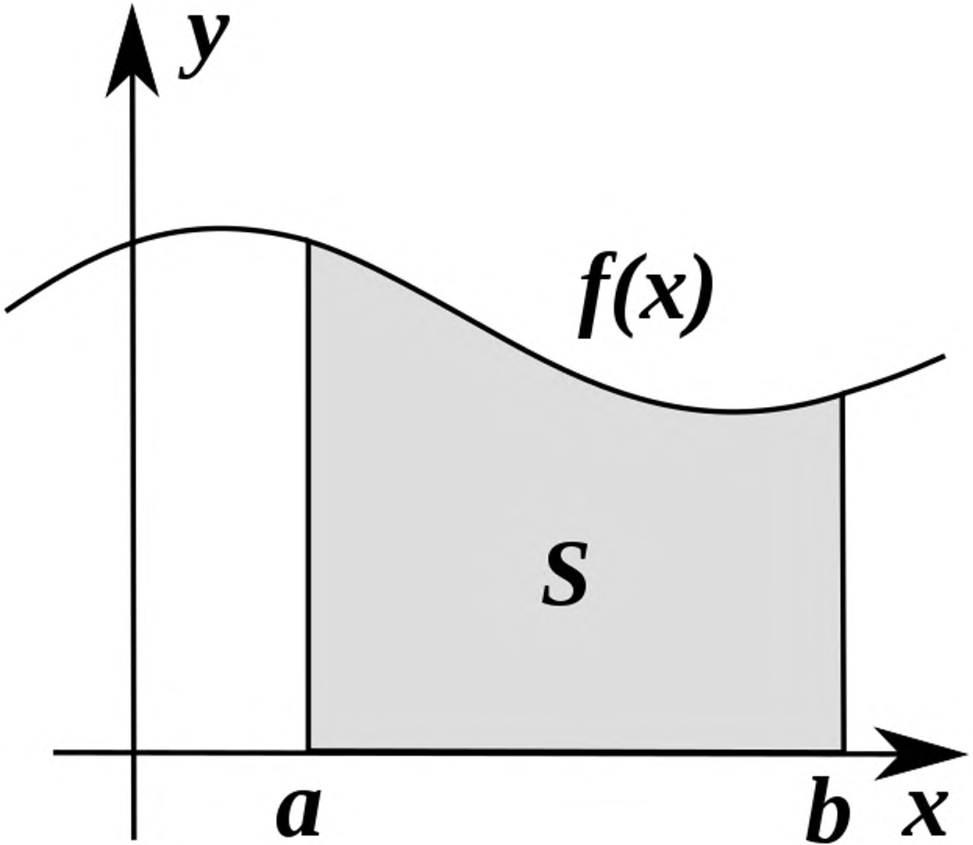
\includegraphics[scale=0.4]{./media/geometric_interpretation_of_density.pdf}}
\end{figure}
\[ P(\xi \in [a,b]) = \int\limits_{a}^{b} p_{\xi} (x) dx \]

Зная плотность вероятности, можно также определить наиболее вероятное значение (моду) случайной величины как максимум $p_{\xi}(x)$. Также с помощью плотности вероятности находится среднее значение случайной величины:
\[ E\xi = \int\limits_{-\infty}^{\infty} x p_{\xi} (x) dx \]

\noindent \textbf{Пример}

Широко известным распределением является «нормальное», оно же гауссово, плотность которого записывается как
\[ p_{\xi} (x) = \frac{1}{\sqrt{2 \pi} \sigma} e^{- \frac{(x - \mu)^2}{2 \sigma^2}} \]
где $\mu$ и $\sigma$ - параметры: математическое ожидание и среднеквадратичное отклонение.

\textit{Стандартным нормальным распределением} называется нормальное распределение с математическим ожиданием $\mu = 0$ и стандартным отклонением $\sigma = 1$.

\section{Как вычислить $P(\xi \in [a, b), \eta \in [c, d))$, зная совместную функцию распределения $F_{\xi\eta}$?}

\[F_{\xi\eta}(b, d) = P(\xi < b, \eta < d)\]
\[F_{\xi\eta}(a, c) = P(\xi < a, \eta < c)\]
Тогда:
\[P(\eta \in [a,b), \xi \in [c,d)) = F_{\xi\eta}(b, d) - F_{\xi\eta}(a, c)\]

\section{Что называют условной вероятностью события $A$ при условии события $B$ (формула)?}

Пусть $A, B$ - события, $P(B) > 0$. Условная вероятность $A$ при условии $B$: $P(A | B) = \dfrac{P(AB)}{P(B)}$

\begin{remark}
	Пусть $B$ - произошло, тогда
	\[ P(B|B) = 1 ~~~~~~ P(A^*|B) = \frac{P(A^*)}{P(B)}, A^* \subset B ~~~~~~ P(A^{**} | B) = 0, A^{**} \cap B = \emptyset \]
	\[ P(\bar B | B) = 0 ~~~~~~ A = AB \cup A \backslash B ~~~~~~ P(A|B) = P(AB | B) + \underset{=0}{P(A \bar B | B)} \]
\end{remark}

\textbf{Свойства:}
\begin{enumerate}
	\item $A \cap B = \emptyset \Rightarrow P(A|B) = 0$
	\item $A \supseteq B \Rightarrow P(A|B) = \dfrac{P(A)}{P(B)}$
	\item $A, B$ - независимы, $P(A|B) = P(A)$
	\item $P_B: \mathcal{F} \to [0,1]$, т.ч. $P_B (A) = P(A|B), A \in \mathcal{F}$
	
	$P_B$ - вероятность (т.е. удовл. АВ1-АВ3)
\end{enumerate}

\section{Что называется функцией распределения случайного вектора?}

Функцию распределения случайного вектора $\xi = (\xi_1, \xi_2, \dots, \xi_d)$ определяем как функцию $F_{\xi}: \mathbb{R}^d \to \mathbb{R}^1$ такую, что для любого $(x_1, \dots, x_d) \in \mathbb{R}^d$
\[ F_{\xi} (x_1, x_2, \dots, x_d) = P(\xi_1 < x_1, \xi_2 < x_2, \dots, \xi_d < x_d) \]

\noindent Через распределение случайного вектора функция распределения выражается так:
\[F_\xi(x_1,\dots,x_d) = \mathcal{P}_\xi((-\infty,x_1]\times(-\infty, x_n]))\]

\textbf{Свойства функции распределения случайного вектора:}

\begin{enumerate}
	\item $0 \le F_{\xi} (x_1, \dots, x_d) \le 1$.
	\item $F_{\xi}$ - непрерывна слева по каждой координате\footnote{Функция $f(x)$ называется непрерывной слева в точке $a$, если $f(a-0) = \lim\limits_{x \to a - 0} f(x) = f(a)$.}.
	\item $F_{\xi} (x_1, \dots, x_k, \dots, x_d) \underset{x_k \to - \infty}{\to} 0$, для любого $k \le d$.
	\item $F_{\xi} (x_1, \dots, x_k, \dots, x_d) \underset{x_k \to \infty}{\to} F_{(\xi_1, \dots, \xi_{k-1}, \xi_{x+1}, \dots, \xi_d)} (x_1, \dots, x_{k-1}, x_{k+1}, \dots, x_d)$, для любого $k \le d$, и
	
	$F_{\xi} (x_1, \dots, x_d) \to 1$, если одновременно все переменные $x_1, x_2, \dots, x_d$ стремятся к бесконечности.
	\item Пусть $d=2$ и пусть $a_1 < b_1, a_2 < b_2$. Тогда
	\[ P( (\xi_1, \xi_2) \in [a_1;b_1) \times [a_2;b_2) ) = F_{\xi} (b_1, b_2) - F_{\xi} (a_1, b_2) - F_{\xi} (b_1, a_2) + F_{\xi} (a_1, a_2) \]
\end{enumerate}

\section{Какие случайные вектора называют дискретными?}

Случайный вектор $\vec{\xi}$ имеет дискретное распределение, если существует такое не более чем счётное множество $A \subset \mathbb{R}^d$, что $P(\xi \in A) = 1$.

Отметим, что следующие два утверждения равносильны:
\begin{enumerate}
	\item $\xi = (\xi_1, \dots, \xi_d)$ - случайный вектор с дискретным распределением.
	\item Для всех $k \le d$ случайные величины $\xi_k$ имеют дискретное распределение.
\end{enumerate}

\section{Что называют плотностью распределения случайного вектора?}

Случайный вектор $\xi$ с абсолютно непрерывным распределением, если существует такая функция $p_{\xi} (x_1, x_2, \dots, x_d)$, что при любом $(y_1, y_2, \dots, y_d)$ справедливо равенство
\[ F_{\vec{\xi}} (y_1, \dots, y_d) = \int_{-\infty}^{y_1} \dots \int_{-\infty}^{y_d} p_{\vec{\xi}} (x_1, \dots, x_d) dx_1 \dots dx_d = \int\limits_{( - \infty; y_1 ] \times \dots \times ( - \infty; y_n ]} p_{\vec{\xi}} (\vec{x}) d \mu_n (\vec{x}) \]
Здесь функция $p_{\vec{\xi}}$ называется \textit{плотностью распределения} случайного вектора, а $\mu_n$ - мера Лебега.

\noindent \textbf{Мера}

\noindent Функция, действующая $\mu: \mathcal{A} \to [0, \infty]$ называется мерой.

\noindent Мера - неотрицательная счётно-аддитивная функция множеств из $\mathcal{A} - \sigma$-алгебра.

\noindent \textbf{Мера Лебега}

\noindent $X = \mathbb{R}, \mathcal{A} = \mathcal{B}_1$, где $\mathcal{B}_1$ - борелевская $\sigma$-алгебра - наименьшая сигма-алгебра, содержащая все интервалы $(a, b], a, b \in \mathbb{R}, b > a$.

\noindent $\mu_1$ - мера Лебега, определённая на интервалах $\mu ((a, b]) = b - a$. По свойствам меры $\mu_1$ продолжается единственным образом на $\mathcal{B}_1$.

\section{Какие случайные величины называют независимыми?}

Пусть на некотором вероятностном пространстве $(\Omega, \mathcal{F}, P)$ определены $\xi_1, \dots, \xi_n$ - случайные величины, $\vec{\xi} = (\xi_1, \dots, \xi_n)$ - соответствующий случайный вектор. $\mathcal{P}_{\xi_1, \dots, \xi_n}$ - распределение ($F_{\xi_1, \dots, \xi_n}$ - ф-я распределения), $p_{\xi_1, \dots, \xi_n}$ - плотность распределения. $B_1, \dots, B_n$ - борелевские подмножества множества вещественных чисел, $B_1, \dots, B_n \in \mathcal{B}$ - множество борелевских подмножеств множества вещественных чисел (борелевская $\sigma$-алгебра).

\textit{В терминах борелевских подмножеств:}

\[ P(\xi_1 \in B_1, \dots, \xi_n \in B_n) = \prod_{i=1}^{n} P(\xi_i \in B_i) \]

\section{Критерий независимости в терминах функций распределения.}

\textit{В терминах распределения случайного вектора:}

\[ \mathcal{P}_{\vec{\xi}} (B_1 \times \dots \times B_n) = \mathcal{P}_{\vec{\xi}} (B_1 \times \mathbb{R} \times \dots \times \mathbb{R}) \cdot \mathcal{P}_{\vec{\xi}} (\mathbb{R} \times B_2 \times \dots \times \mathbb{R}) \cdot ... \cdot \mathcal{P}_{\vec{\xi}} (\mathbb{R} \times ... \times \mathbb{R} \times B_n) \]

\textit{В терминах функций распределения:}

Говорим, что $\xi_1, \dots, \xi_n$ - независимые случайные величины, если для любых $x_1, x_2, \dots, x_n \in \mathbb{R}$ при условии совпадения всех функций распределений справедливо равенство:

\[ F_{\vec{\xi}} (x_1 \dots x_n) = \underset{F_{\vec{\xi}}(x_1, \infty, \dots, \infty)}{F_{\xi_1}(x_1)} \cdot ... \cdot \underset{F_{\vec{\xi}}(\infty, \dots, \infty, x_n)}{F_{\xi_n}(x_n)} = \prod_{i=1}^{n} F_{\xi_i} (x_i) \]
Это означает, что
\[ P(\xi_1 < x_1, \dots, \xi_n < x_n) = \prod_{i=1}^{n} P(\xi_i < x_i) \]
Заметим, что здесь речь идет о независимости в совокупности.

\section{Критерий независимости в терминах плотностей.}

\textit{В терминах плотностей:}

Для абсолютно непрерывных величин независимость можно задать в терминах плотностей: для любых $x_1, x_2, \dots, x_n \in \mathbb{R}$:
\[ p_{\vec{\xi}} (x_1 \dots x_n) = p_{\xi_1} (x_1) \dots p_{\xi_n} (x_n) \]
\[ p_{\xi_i} (x_i) = \int_{\mathbb{R}^{n-1}} p_{\vec{\xi}} (\vec{x}) dx_1 \dots dx_{i-1} dx_{i+1} \dots dx_n \]

\section{Что называется условной функцией распределения случайного вектора $\xi$ при условии $\eta$?}

\noindent \textbf{Дискретный случай}
Пусть $\xi = (\xi_1,\dots,\xi_n)$ - случайный вектор, $\xi = (\eta_1, \eta_2)$, где $\eta_1=(\xi_1,\dots,\xi_k), \eta_2=(\xi_{k+1},\dots,\xi_n)$.

Пусть $\eta_1=y$ - известен. Условное распределение $\eta_2$ при условии $\eta_1$?
\[a_i=(b_{1i}, b_{2i})\]
\[P(\eta_2=b_{2i} | \eta_1=b_{1i})=\dfrac{P(\xi=a_i)}{\underbrace{P(\eta_1=b_{1i})}_{>0}} = \dfrac{P(\eta_2=b_{2i}, \eta_1=b_{1i})}{\underbrace{P(\eta_1=b_{1i})}_{>0}} \]
Тогда функция распределения
\[F(\eta_2 | \eta_1 = b_{1i})(b_{2i}) = P(\eta_2 < b_{2i} | \eta_1=b_{1i}) =  \sum\limits_{k<b_{2i}} P(\eta_2 = k | \eta_1=b_{1i})\]


\noindent \textbf{Абсолютно непрерывный случай}
Пусть $(\xi_1, \xi_2)$ - случайные величины (векторы), $p_{\vec{\xi}}(x,y)$ - плотность совместного распределения.

\[p_{\xi_1}(x)=\int_{-\infty}^{\infty} p_{\vec{\xi}}(x,y)dy \text{ - плотность распределения } \xi_1\]
\[p_{\xi_2|\xi_1=x}(y)=\dfrac{p_\xi(x,y)}{\underbrace{p_{\xi_1}(x)}_{>0}}, y\in \mathbb{R}, x \text{ - фиксированный}\]
Для определенности положим, что $\xi_2=(\xi_{21}, \dots, \xi_{2n})$. Тогда условная функция распределения (в абс. непрерывном случае)
\[F_{\xi_2|\xi_1=x}(y)=\int\limits_{-\infty}^{y_1} \dots \int\limits_{-\infty}^{y_n} p_{\xi_2|\xi_1=x}(y)dy\]

\section{Что называется условной плотностью распределения случайного вектора $\xi$ при условии $\eta$?}

Пусть $\xi = (\xi_1,\dots,\xi_n)$ - случайный вектор, $\xi = (\eta_1, \eta_2)$, где $\eta_1=(\xi_1,\dots,\xi_k), \eta_2=(\xi_{k+1},\dots,\xi_n)$.

Пусть $\eta_1=y$ - известен. Условное распределение $\eta_2$ при условии $\eta_1$?

\noindent \textbf{Абсолютно непрерывный случай}
Пусть $(\xi_1, \xi_2)$ - случайные величины (векторы), $p_{\vec{\xi}}(x,y)$ - плотность совместного распределения.

\[p_{\xi_1}(x)=\int_{-\infty}^{\infty} p_{\vec{\xi}}(x,y)dy \text{ - плотность распределения } \xi_1\]
\[p_{\xi_2|\xi_1=x}(y)=\dfrac{p_\xi(x,y)}{\underbrace{p_{\xi_1}(x)}_{>0}}, y\in \mathbb{R}, x \text{ - фиксированный}\]

\section{Вычисление распределения суммы независимых случайный величин. Формула свёртки.}

Предположим, что $\xi, \eta$ - независимые случайные величины с известными нам функциями распределения $F_{\xi}, F_{\eta}$. Как вычислить $P(\xi + \eta \in D)$, где $D$ - произвольное измеримое подмножество вещественной прямой\footnote{Напомним, что борелевская сигма-алгебра - это минимальная сигма-алгебра, содержащая все открытые подмножества топологического пространства (впрочем, она содержит и все замкнутые). Обычно в качестве топологического пространства выступает множество вещественных чисел.}? Известно, что
\[ P(\xi + \eta \in D) = \int_{D} d F_{\xi + \eta} (x) \]


\[ p_{(\xi + \eta)} (x) = \int\limits_{-\infty}^{\infty} p_{\xi} (x - y) p_{\eta} (y) dy = \int\limits_{-\infty}^{\infty} p_{\eta} (x - y) p_{\xi} (y) dy. \]
		Данная формула называется \textbf{формулой свертки для плотностей}.
\begin{center}
	\textbf{Формула свертки для функций распределения}
\end{center}
\[ F_{\xi + \eta} (x) = \int\limits_{-\infty}^{\infty} F_{\xi} (x - y) d F_{\eta} (y) = \int\limits_{-\infty}^{\infty} F_{\eta} (x - y) d F_{\xi} (y) \]

\section{Мат. ожидание и его свойства.}

Математическим ожиданием случайной величины $\xi$ называют \textbf{число} $E\xi$, определяемое равенством
\[ E\xi = \int_{\omega \in \Omega} \xi (\omega) d P(\omega) = \int_{-\infty}^{\infty} x dF_{\xi} (x) = 
\left[
\begin{array}{c}
	\sum\limits_{i: p_i > 0} a_i p_i, p_i = P(\xi = a_i), \sum_{i} p_i = 1 \text{ (дискретное)} \\
	\int\limits_{\mathbb{R}} x p_{\xi} (x) dx, p_{\xi} - \text{ плотность распределения } \xi (\exists \text{ если } \int \text{ сход.})
\end{array}
\right.
\]
где $F_{\xi}$ - функция распределения величины $\xi$.
Если оно (это число) существует. Если интеграл расходится, то говорят, что у случайной величины отсутствует математическое ожидание.

\begin{remark}
	Математическое ожидание часто еще называют средним случайной величины. Предположим, что у случайной величины $\xi$ ровно $n$ значений, и все $p_i = \frac{1}{n}$, тогда $\xi = \frac{1}{n} \sum\limits_{i} a_i$ - среднее арифметическое значений случайной величины.
\end{remark}

\noindent \textbf{Свойства математического ожидания}
	
\begin{enumerate}
	\item Если $P(\xi = c) = 1$, то $E\xi = c$.
	\item Линейность математического ожидания. Пусть $\xi, \eta$ - случайные величины. Тогда для любых $\alpha, \beta \in \mathbb{R}$ справедливо равенство: $E(\alpha \xi + \beta \eta) = \alpha E \xi + \beta E \eta$. В данном случае предполагаем, что математические ожидания, о которых идет речь, существуют.
	\item Если $P(\xi \ge 0) = 1$, то $E\xi \ge 0$.
	\item Если $P(\xi \ge \eta) = 1$, то $E\xi \ge E\eta$.
	\item Справедливо неравенство $|E\xi| \le E |\xi|$.
\end{enumerate}

\section{Дисперсия и её свойства.}

Дисперсией случайной величины $\xi$ называется центральный момент второго порядка $E(\xi - E\xi)^2$, если этот момент существует.

Стандартное обозначение для дисперсии - $D\xi$.

Из определения математического ожидания следует, что
\[ D\xi = \int_{\Omega} ( \xi (\omega) - E\xi )^2 d P(\omega) \]

Таким образом, дисперсия — это среднее значение квадрата отклонения случайной величины от её математического ожидания.

\noindent \textbf{Свойства дисперсии}
\begin{enumerate}
	\item $D\xi \ge 0$ и $D\xi = 0$ тогда и только тогда, когда $P(\xi = c) = 1$ для некоторого $c \in \mathbb{R}$ (т.е. случайная величина $\xi$ имеет вырожденное распределение).
	\item Если $\alpha, \beta \in \mathbb{R}$, то $D(\alpha \xi + \beta) = \alpha^2 D\xi$
	\item $D\xi = E\xi^2 - (E\xi)^2$
	\item $D(\xi + \eta) = D\xi + D\eta + 2E (\xi - E\xi) (\eta - E\eta)$
	\item Если $\xi$ и $\eta$ - независимые случайные величины и существуют их дисперсии, то $D(\xi + \eta) = D\xi + D \eta$. Верно и для произвольного числа попарно независимых случайных величин. В обратную сторону неверно.
\end{enumerate}
\begin{remark}
	Дисперсия разности: $D(\xi - \eta) = D\xi + D(-\eta) = D\xi + D\eta$, т.е. дисперсия разности – это НЕ разность дисперсий.
\end{remark}

\section{Что называется условным мат. ожиданием $\xi$ при условии $\eta$, если $(\xi, \eta)$ абс. непр. случайный вектор?}

\[E(\xi|\eta=x)=\int_{-\infty}^{\infty} y \cdot p_{\xi|\eta=x}(y)dy = f(x) \text{ - зависит от значения фиксированного } x\]
Условное ожидание случайной величины $\xi$ относительно $\eta$:
\[E(\xi|\eta)=E(\xi|\eta=x)|_{\xi=x}=f(\eta) \text{ - то же самое, но зависит от } \eta\]

\section{Что называется условным мат. ожиданием $\xi$ при условии $\eta$, если $(\xi, \eta)$ - дискретный случайный вектор?}
Если $(\xi, \eta)$ - дискретный вектор, то $\xi, \eta$ - дискретные величины. Условное мат ожидание $\xi$ при условии $\eta$:
\[E(\xi | \eta=y) = \sum \limits_{i=1}^{\infty} x_i P(\xi = x_i | \eta=y)\]
\section{Свойства условных мат. ожиданий.}

\[f(\eta)=E(\xi|\eta)\]
\begin{enumerate}
	\item $E(E(\xi|\eta))=E\xi$
	\item Если $\xi, \eta$ - независимые, то $E(\xi|\eta)=E\xi$
	\item $E(g(\xi)|\xi)=g(\xi)$, если $g$ - фиксированная изначально функция
	\item $E(\xi\eta|\xi)=\xi E(\eta|\xi)$
	\item $E(\xi|\eta)=E(E(\xi|(\eta,\nu))|\eta), \forall \xi,\eta=E((E|\xi|\eta)|(\eta,\nu))$
\end{enumerate}

\begin{remark}
	Смотри 217 стр. Ананьевский
\end{remark}

\section{Что такое ковариация и коэффициент корреляции?}

\noindent \textbf{Ковариация}

Пусть $(\Omega, \Event, P)$ - вероятностный эксперимент, а $\xi, \eta$ - случайные величины, определённые в нём.

\noindent Смешанный центральный момент второго порядка
\[ E (\xi - E\xi) (\eta - E\eta) = \cov (\xi, \eta) \]
называется ковариацией случайных величин $\xi$ и $\eta$.

Для ковариации выполняются следующие свойства:
\begin{enumerate}
	\item $\cov (\xi, \eta) = E \xi \eta - E \xi E \eta$;
	\item Если $\xi, \eta$ - независимые случайные величины, то $\cov (\xi, \eta) = 0$;
	
	Обратное утверждение — неверное.
	
	\item Если $a, b$ - числа, то $\cov (a \xi + b, \eta) = a \cov (\xi, \eta)$.
\end{enumerate}

\noindent \textbf{Коэффициент корреляции}

Пусть $\xi, \eta$ - случайные величины, у которых существуют дисперсии и $D\xi D\eta > 0$. Тогда число
\[ \rho (\xi, \eta) = \frac{\cov (\xi, \eta)}{\sqrt{D\xi \cdot D\eta}} \]
называется коэффициентом корреляции случайных величин $\xi$ и $\eta$.

\section{Свойства ковариации и коэффициента корреляции}

\noindent \textbf{Ковариация}

Пусть $(\Omega, \Event, P)$ - вероятностный эксперимент, а $\xi, \eta$ - случайные величины, определённые в нём.

\noindent Смешанный центральный момент второго порядка
\[ E (\xi - E\xi) (\eta - E\eta) = \cov (\xi, \eta) \]
называется ковариацией случайных величин $\xi$ и $\eta$.

Для ковариации выполняются следующие свойства:
\begin{enumerate}
	\item $\cov (\xi, \eta) = E \xi \eta - E \xi E \eta$;
	\item Если $\xi, \eta$ - независимые случайные величины, то $\cov (\xi, \eta) = 0$;
	
	Обратное утверждение — неверное.
	
	\item Если $a, b$ - числа, то $\cov (a \xi + b, \eta) = a \cov (\xi, \eta)$.
\end{enumerate}

\noindent \textbf{Коэффициент корреляции}

Пусть $\xi, \eta$ - случайные величины, у которых существуют дисперсии и $D\xi D\eta > 0$. Тогда число
\[ \rho (\xi, \eta) = \frac{\cov (\xi, \eta)}{\sqrt{D\xi \cdot D\eta}} \]
называется коэффициентом корреляции случайных величин $\xi$ и $\eta$.

Для коэффициента корреляции выполняются следующие свойства.

\begin{enumerate}
	\item Справедливы неравенства:
	\[ -1 \le \rho (\xi, \eta) \le 1 (\text{т.е. } |\rho(\xi, \eta)| \le 1) \]
	\item Если $\xi, \eta$ - независимые случайные величины, то $\rho (\xi, \eta) = 0$. (Обратное утверждение - неверное.)
	\item Если $|\rho(\xi, \eta)| = 1$, то это означает, что существуют числа $a \ne 0$ и $b$ такие, что $P(\xi = a\eta + b) = 1$ (т.е. $\xi$ и $\eta$ - линейно связные с вероятностью единица величины), и $a \rho(\xi, \eta)>0$ (т.е. знак $a$ совпадает со знаком коэффициента корреляции).
\end{enumerate}

\noindent \textbf{Дополнительно:}

\href{http://www.machinelearning.ru/wiki/index.php?title=%D0%9A%D0%BE%D0%B2%D0%B0%D1%80%D0%B8%D0%B0%D1%86%D0%B8%D0%BE%D0%BD%D0%BD%D0%B0%D1%8F_%D0%BC%D0%B0%D1%82%D1%80%D0%B8%D1%86%D0%B0}{Сайт} с этим и другим трэшем.

Ковариационная матрица - матрица, составленная из попарных ковариаций элементов одного или двух случайных векторов.
\[
\vec{\xi} =
\begin{pmatrix}
	r_{11} & \dots & r_{1n} \\
	\dots  & \dots & \dots \\
	r_{n1} & \dots & r_{nn}
\end{pmatrix},
r_{ij} = \cov (\xi_i, \xi_j)
\]

\textit{Ковариационная матрица случайного вектора} — квадратная симметрическая неотрицательно определенная матрица, на диагонали которой располагаются дисперсии компонент вектора, а внедиагональные элементы — ковариации между компонентами.

\textit{Корреляционная матрица} — матрица коэффициентов корреляции нескольких случайных величин с ненулевыми дисперсиями.

\noindent В которой элементы $r_{ij} = \frac{\cov (\xi_i, \xi_j)}{\sqrt{D\xi_i} \sqrt{D\xi_j}}$ есть коэффициенты корреляции соответствующих случайных величин. Диагональные элементы матрицы равны единице.

\section{Неравенство Йенсена для мат. ожидания.}

Если $E\xi$ существует и $g(x)$ - выпуклая вниз функция, то $g(E\xi) \le E g(\xi)$.

\section{Неравенства Чебышева и где они применяются.}

Для произвольной случайной величины $\xi$, имеющей математическое ожидание, справедливо неравенство
\[ P( |\xi - E\xi| \ge \epsilon ) \le \frac{D\xi}{\epsilon^2} \]
при $D\xi < \infty$ и $\xi > 0$.

\noindent \textbf{Применение:}

\begin{itemize}
	\item С помощью неравенства Чебышева мы имеем возможность оценивать вероятности различных уклонений $\xi$ (от мат. ожидания), зная лишь $E\xi$ и $D\xi$.
	\item Из данного нер-ва можно получить так называемый закон больших чисел в форме Чебышева.
\end{itemize}

\noindent Другая форма записи нер-ва Чебышева (используется реже):

\[ g: \mathbb{R}_{+} \to \mathbb{R}_{+} - \text{ неотрицательная, неубывающая функция} \]
\[ \text{Случайная величина } \xi : P(\xi > 0) = 1, ~~~~~~ Eg(\xi) < \infty, g(x) > 0, x > 0 \]
\[ P (|\xi| > \epsilon) \le \frac{Eg(\xi)}{g(\xi)} \]

\section{Неравенство Гёльдера для мат. ожидания.}

Если $r, s > 0$ и $\frac{1}{r} + \frac{1}{s} = 1$, то
\[ E |\xi \eta| \le (E|\xi|^r)^{\frac{1}{r}} ( ( E |\eta|^s )^{\frac{1}{s}} ) \]
для любых случайных величин $\xi, \eta$ (если соответствующие моменты существуют).

\section{Неравенство Минковского для мат. ожидания.}

Если $p, q > 0$ и $\frac{1}{p} + \frac{1}{q} = 1$, то
\[ ( E |\xi + \eta|^p )^{\frac{1}{p}} \le ( E |\xi|^p )^{\frac{1}{p}} + ( E |\eta|^p )^{\frac{1}{p}} \]
для любых случайных величин $\xi, \eta$.

\section{Неравенство Ляпунова для мат. ожидания.}

Если $p < q$, то $(E |\xi|^p)^{\frac{1}{p}} \le (E |\xi|^q)^{\frac{1}{q}}$. (Это свойство можно сформулировать иначе: введем функцию $g_{\xi}(p) = (E |\xi|^p)^{\frac{1}{2}}$, тогда $g_{\xi}(p)$ не убывает).

\section{Неравенство Коши-Буняковского для мат. ожидания.}

\textbf{Неравенство Коши–Буняковского–Шварца} (частный случай неравенства Гёльдера при $p=q=2$).

Если положим $p = q = 2$, то неравенство Гёльдера будет иметь следующий вид:
\[ E |\xi \eta| \le ( E |\xi|^2 )^{\frac{1}{2}} \cdot ( E |\eta|^2 )^{\frac{1}{2}} \]

\section{Что означает $\xi_n \to \xi$ по вероятности?}

Будем говорить, что последовательность случайных величин $\xi, \xi_1, \xi_2, \dots$ сходится к случайной величине $\xi$ по вероятности (обозначение: $\xi_n \overset{P}{\to} \xi$), если
\[ P(|\xi_n - \xi| \ge \epsilon) \underset{n \to \infty}{\to} 0 \]
для любого $\epsilon > 0$.

\section{Что означает $\xi_n \to \xi$ с вероятностью 1?}

Будем говорить, что последовательность случайных величин $\xi_1, \xi_2, \dots$ сходится к случайной величине $\xi$ почти наверное или с вероятностью 1 (обычно обозначается $\xi_n \to \xi$ п.н.), если верно равенство
\[ P(\omega : \lim \xi_n (\omega) = \xi (\omega)) = 1 \]

\section{Что означает $\xi_n \to \xi$ в среднеквадратическом?}

Будем говорить, что последовательность случайных величин $\xi_1, \xi_2, \dots$ сходится к случайной величине $\xi$ в среднем порядка $p$ (обозначение: $\xi_n \overset{L_p}{\to} \xi$), если существует $E\xi^p$ и $E\xi_n^p$ и имеет место сходимость:
\[ E |\xi - \xi_n|^p \underset{n \to \infty}{\to} 0 \]

В среднеквадратическом - значит в среднем порядка 2.

\section{Какая связь между сходимостью по вероятности, с вероятностью 1 и в среднем?}

Пусть:
\begin{enumerate}
	\item Сходимость по вероятности.
	\item Сходимость с вероятностью 1 или почти наверное.
	\item Сходимость в среднем порядкe $p(p > 0)$.
	\item Сходимость по распределению.
\end{enumerate}

Имеют место следующие соотношения:
\[ 2 \Rightarrow 1, 3 \Rightarrow 1, 1 \Rightarrow 4, \]
т.е. из сходимости почти наверное следует сходимость по вероятности, из сходимости в среднем следует сходимость по вероятности и из сходимости по вероятности следует сходимость по распределению.
\begin{figure}[H]
	\center{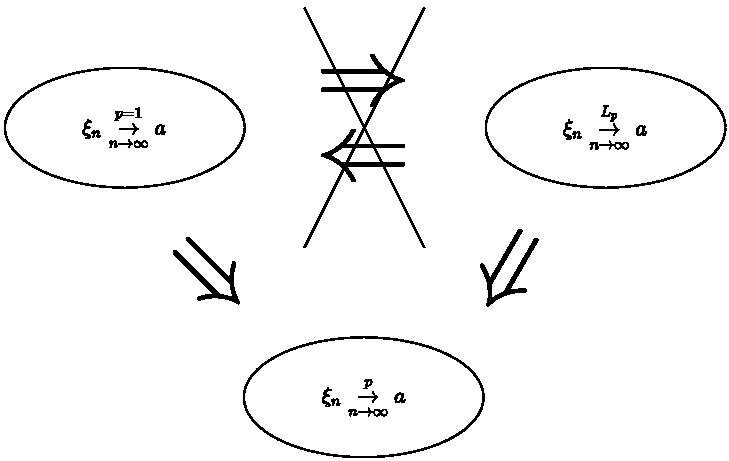
\includegraphics[scale=1]{./media/relationship_between_convergence.pdf}}
\end{figure}

\noindent \textbf{Критерий сходимости почти наверное}

Пусть $\xi_1,\xi_2,\dots$ - случайные величины на $(\Omega, \mathcal{F},P)$, тогда:
\[\xi_n \overset{\text{п.н.}}{\rightarrow } \xi \Leftrightarrow \forall \epsilon > 0: P(sup_{k\ge n} |\xi_k-\xi| > \epsilon) \rightarrow 0, n \rightarrow \infty\]

Именно из этого критерия получаем, что из сходимости почти наверное следует сходимость по вероятности.
\begin{remark}
	Доказательство этого смотри в Ананьевский - стр. 116 - Теорема 4.2.1.
\end{remark}

\section{Определение слабой сходимости.}

Будем говорить, что последовательность случайных величин $\xi_1, \xi_2, \dots$ сходится к случайной величине $\xi$ по распределению (обозначение: $\xi_n \overset{d}{\to} \xi$), если
\[ F_{\xi_n} (x) \underset{n \to \infty}{\to} F_{\xi} (x) \]
для любой $x$ - точки непрерывности функции $F_{\xi}$.

\section{Теорема Маркова о законе больших чисел.}

Пусть $\xi_1, \xi_2, \dots$ - случайные величины и пусть при всех $n \ge 1$ существуют дисперсии $D \left( \sum\limits_{k=1}^{n} \xi_k \right)$. Кроме того, пусть
\[ \frac{1}{n^2} D \left( \sum\limits_{k=1}^{n} \xi_k \right) \underset{n \to \infty}{\to} 0 \]
Тогда для данной последовательности выполняется закон больших чисел.

\section{Теорема Чебышева о законе больших чисел.}

\noindent \textbf{Неравенство Чебышева}

Для произвольной случайной величины $\xi$, имеющей математическое ожидание, справедливо неравенство
\[ P( |\xi - E\xi| \ge \epsilon ) \le \frac{D\xi}{\epsilon^2} \]

\begin{remark}
	С помощью неравенства Чебышева мы имеем возможность оценивать вероятности различных уклонений $\xi$, зная лишь $E\xi$ и $D\xi$.
\end{remark}

\noindent \textbf{ЗБЧ Чебышёва}

Пусть $\xi_1, \xi_2, \dots$ - попарно независимые случайные величины и пусть для всех $k = 1, 2, \dots$ существуют и равномерно ограничены дисперсии случайных величин, т.е. $\sigma_k^2 = D\xi_k \le c$, где $c$ - некоторая неотрицательная константа. Тогда для данной последовательности случайных величин выполняется закон больших чисел.
\begin{proof}
	Утверждение сразу следует из теоремы Маркова, если учесть, что в данной ситуации
	\[ \frac{1}{n^2} D \left( \sum_{k=1}^{n} \xi_k \right) = \frac{1}{n^2} \sum_{k=1}^{n} \sigma_k^2 \le \frac{n \cdot c}{n^2} \underset{n \to \infty}{\to} 0 \]
\end{proof}

\noindent \textbf{Следствия из теоремы Чебышёва}
	
1. Если $\xi_1, \xi_2, \dots$ - независимые одинаково распределенные случайные величины и при всех $k \ge 1$ существуют дисперсии $D\xi = \sigma^2 > 0$, то выполняется ЗБЧ.

\noindent 2. Пусть $\xi_1, \xi_2, \dots$ - независимые одинаково распределенные случайные величины, принимающие значения 0 и 1 с вероятностями $(1-p)$ и $p$, соответственно. Тогда
\[ \frac{1}{n} \sum_{k-1}^{n} \xi_k \overset{P}{\to} p \]

Заметим, что следствие 2 можно рассматривать как теорему о законе больших чисел для испытаний Бернулли.

\section{Что называется законом больших чисел и его запись с использованием известных видов сходимости последовательностей случайных величин.}

Пусть $\xi_1, \xi_2, \dots$ - последовательность случайных величин, с математическими ожиданиями $a_k = E\xi_k, k = 1, 2, \dots$. Будем говорить, что для последовательности случайных величин выполняется закон больших чисел, если имеет место сходимость
\[ \frac{1}{n} \sum_{k=1}^{n} (\xi_k - a_k) \overset{P}{\to} 0 \]
Это означает, что
\[ P \left( \left| \frac{1}{n} \sum_{k=1}^{n} \xi_k - \frac{1}{n} \sum_{k=1}^{n} a_k \right| \ge \epsilon \right) \underset{n \to \infty}{\to} 0 \]
или, что то же самое,
\[ P \left( \left| \frac{1}{n} \sum_{k=1}^{n} (\xi_k - a_k) \right| \ge \epsilon \right) \underset{n \to \infty}{\to} 0 \]
для любого $\epsilon > 0$.

В записи закона используется сходимость по вероятности.

ЗБЧ утверждает, что среднее значение случайных величин из заданного распределения близко к теоретическому среднему значению (математическое ожидание) этого распределения

На неформальном языке закон можно трактовать так: при увеличении числа испытаний частота появления события будет все меньше отличаться от вероятности его появления.

\section{Сформулировать ЦПТ Леви в частном случае испытаний Бернулли.}

\noindent \textbf{Интегральная теорема Муавра—Лапласа}

Пусть $\xi_1, \xi_2, \dots$ - последовательность независимых одинаково распределенных случайных величин, с распределением Бернулли, то есть $P (\xi_k = 1) = 1 - P(\xi_k = 0) = p$, где $0 < p < 1$.

Каждую из случайных величин $\xi_k$ можем интерпретировать как результат при $k$-ом испытании. Если случайная величина $\xi_k$ приняла значение 1, то это означает, что в $k$-м испытании произошел "успех"\,, если $\xi_k$ приняла значение 0, то в $k$-м испытании "неудача"\,. Тогда $\sum\limits_{k=1}^{n} \xi_k$ означает число "успехов" в $n$ испытаниях. Для этих случайных величин $E\xi_k = p, D\xi_k = p(1-p)$. Тогда выполнены условия теоремы Леви, и, следовательно, выполняется указанное соотношение для всех $x \in \mathbb{R}$. Можно для любых $a, b \in \mathbb{R}$ написать, что
\[ P \left( a \le \frac{\sum\limits_{k=1}^{n} \xi_k - np}{\sqrt{np (1-p)}} < b \right) - \frac{1}{\sqrt{2 \pi}} \int_{a}^{b} e^{- \frac{u^2}{2}} du \underset{n \to \infty}{\to} 0 \]
или
\[ P \left( a \le \frac{\sum\limits_{k=1}^{n} \xi_k - np}{\sqrt{np (1-p)}} < b \right) - (\Phi(b) - \Phi(a)) \underset{n \to \infty}{\to} 0 \]
Осталось учесть монотонность и поведение на бесконечностях функций распределения, что приводит к окончательному выводу, фиксирующему наличие равномерной сходимости:
\[ \sup_{a < b} \left| P \left( a \le \frac{\sum\limits_{k=1}^{n} \xi_k - np}{\sqrt{np (1-p)}} < b \right) - (\Phi(b) - \Phi(a)) \right| \underset{n \to \infty}{\to} 0 \]

\section{Центральная предельная теорема Леви.}

Пусть $\xi_1, \xi_2, \dots$ - последовательность независимых одинаково распределенных случайных величин, у которых существует математическое ожидание $a = E\xi_k$ и существует конечная дисперсия $\sigma^2 = D\xi_k > 0$. Тогда, для всех $x \in \mathbb{R}$ имеет место сходимость
\[ P \left( \frac{\sum\limits_{k=1}^{n} \xi_k - na}{\sqrt{n \sigma^2}} < x \right) \underset{n \to \infty}{\to} \Phi (x) = \frac{1}{\sqrt{2 \pi}} \int_{- \infty}^{\infty} e^{- \frac{u^2}{2}}du \]
(Это предельное соотношение записывают ещё следующим образом:
\[ \frac{\sum\limits_{k=1}^{n} \xi_k - na}{\sqrt{n \sigma^2}} \overset{d}{\to} \mathcal{N} (a, \sigma^2) ) \]

\section{Последовательность независимых случайных величин (НСВ) и марковские последовательности. Примеры марковских последовательностей, построенных по последовательности НСВ.}

\noindent\textbf{Марковское свойства:}
\[ p(\xi_{k+1} \in A_{k+1} | \xi_1 = x_1, \dots, \xi_k = x_k) = p (\xi_{k+1} \in A_{k+1} | \xi_k = x_k),\]
\[\forall x_1, \dots, x_k \in \mathbb{R} (\text{почти наверное}), \forall A_{k+1} \in \mathcal{B}_1, k \in \mathbb{N} \]

\noindent \textbf{Цепь Маркова}

Цепь Маркова - последовательность случайных величин, удовлетворяющих Марковскому свойству.
\[ E = \bigcup_{i \in \mathbb{N}} supp(\xi_i) - \text{ не более, чем счётное множество состояний ЦМ} \]
\[E={1,\dots,k}, E=\mathbb{N}\]
$E$ - \textit{множество состояний} цепи Маркова.

\begin{enumerate}
	\item $\xi_1, \xi_2, \dots$ - дискретные независимые случайные величины образуют цепь Маркова
	\item Суммы $\xi_1, \xi_2, \dots$ - дискретных независимых случайных величин вида $\eta_k = \sum\limits_{i=1}^k \xi_i$, то есть последовательность $\eta_1, \eta_2, \dots$ - тоже образует цепь Маркова.
	\item $\xi_1, \xi_2, \dots$ - независимые одинаково распределенные случайные величины. Последовательность $\eta_k = \sum\limits_{i=1}^k \xi_i$ - случайное блуждание, когда $P(\xi_1 =1)=p, P(\xi_1=-1)=(1-p)$

	\[
	P = 
	\begin{pmatrix}
		\ldots       & \ddots & p   & 0 & \hdotsfor{3} \\
		\ldots       & 1-p    & 0   & p & 0 & \hdotsfor{2} \\
		\ldots       & 0      & 1-p & 0 & p & 0 & \ldots \\
		\hdotsfor{2} & 0      & 1-p & 0 & p & 0 \\
		\hdotsfor{3} & 0      & 1-p & 0 & p \\
		\hdotsfor{4} & 0      & 1-p & \ddots
	\end{pmatrix}
	\]
\end{enumerate}

\section{Критерий возвратности для цепей Маркова.}

\noindent Если $\exists j: i \to j$, но $j \not\to i$, то $j$ - \textbf{несущественное}; в противном случае $j$ - существенное.

\noindent Состояние $i$ \textit{эргодичное}, если среднее время возвращения конечно
\[ E \tau_i = \sum_{s=1}^{\infty} s f_{ii}^{(s)} < \infty, \]
где $\tau_i$ - время 1-ого возвращения в состояние $i$.

\begin{enumerate}
	\item Несущественные состояния невозвратны;
	\item Состояние $i$ возвратно (т.е. $f_i=1$) $\eq \sum\limits_{s=1}^{\infty} p_{ii}^{(s)} = \infty$
	\item Состояние $i$ возвратно, но не эргодическое $\eq \sum\limits_{s=1}^{\infty} p_{ii}^{(s)} = \infty ~ \& ~ \lim\limits_{s \to \infty} p_{ii}^{(s)} = 0$
	\item Состояние эргодическое $\eq \sum\limits_{s=1}^{\infty} p_{ii}^{(s)} = \infty ~ \&$ не выполнено $\lim\limits_{s \to \infty} p_{ii}^{(s)} = 0$
\end{enumerate}

\section{Марковское свойство, что называется цепью Маркова и уравнение Маркова.}

\noindent Пусть $\xi_1, \dots, \xi_n, \dots$ - случайная последовательность (последовательность случайных величин).

\noindent \textbf{Конечномерное распределение (КМР)}

Распределение последовательности определяют конечномерные распределения
\[ \mathcal{P}_{\xi_1, \dots, \xi_k} (A_1 \times \dots \times A_k) = p(\xi_1 \in A_1, \dots, \xi_k \in A_k), k \in \mathbb{N} \]

\noindent\textbf{Условие согласования:}
\[ p(\xi_1 \in A_1, \dots, \xi_{k-1} \in A_{k-1}) = \mathcal{P}_{(\xi_1, \dots, \xi_k)} (A_1 \times \dots A_{k-1} \times \mathbb{R}) \]
\noindent\textbf{Марковское свойства:}
\[ p(\xi_{k+1} \in A_{k+1} | \xi_1 = x_1, \dots, \xi_k = x_k) = p (\xi_{k+1} \in A_{k+1} | \xi_k = x_k),\]
\[\forall x_1, \dots, x_k \in \mathbb{R} (\text{почти наверное}), \forall A_{k+1} \in \mathcal{B}_1, k \in \mathbb{N} \]

\noindent\textbf{Цепь Маркова}

Цепь Маркова - последовательность случайных величин, удовлетворяющих Марковскому свойству.
\[ E = \bigcup_{i \in \mathbb{N}} supp(\xi_i) - \text{ не более, чем счётное множество состояний ЦМ} \]
\[E={1,\dots,k}, E=\mathbb{N}\]
$E$ - \textit{множество состояний} цепи Маркова.

\noindent\textbf{Уравнение} Маркова (формула полной вероятности)
\[ p_{i,j}^{r+s} = \sum_{k \in E} p_{ik}^{(r)} p_{kj}^{(s)}, \forall i,j \in E; r,s \in \mathbb{N} \]
Вывод: в однородной цепи Маркова
\[ p^{(s)} = || p_{ij}^{(s)} || = \underbrace{P \times ... \times P}_{*} = p^s, * - s \text{ раз умножение матрицы \linebreak по правилам матричного умножения} \]

Структуру однородной цепи Маркова характеризует матрица вероятностей перехода (МВП) или граф.
\begin{enumerate}
	\item (Случайное блуждание) Заданы начальные распределения вероятностей:
	\[
	q_i =
	\begin{cases}
		1, &i = 0 \\
		0, &i \ne 0
	\end{cases}
	~~~~~~
	E = \mathbb{Z} \text{ и МВП }
	p_{ij} =
	\begin{cases}
		p, &j = i + 1 \\
		1 - p, &j = i - 1 \\
		0, j \notin \{i-1,i+1\}\}
	\end{cases}
	\]
\end{enumerate}

\section{Уравнение эргодичности неприводимой цепи Маркова и вычисление финальных вероятностей.}

\noindent Вероятность возвращения на $s$-м шаге впервые
\[ f_{ii}^{(s)} = p (\xi_{k + s} = i, \xi_{k+s-1} \ne i, \dots, \xi_{k+1} \ne i | \xi_k = i) \]
Вероятность возвращения в состояние $i$:
\[ f_i = \sum_{s=1}^{\infty} f_{ii}^{(s)} \le 1 \]
\textbf{(!)} Состояние $i$ \textit{возвратное}, если вероятность возвращения $f_i = 1$.

Состояние $i$ \textit{эргодичное}, если среднее время возвращения конечно
\[ E \tau_i = \sum_{s=1}^{\infty} s f_{ii}^{(s)} < \infty, \]
где $\tau_i$ - время 1-ого возвращения в состояние $i$.

\textbf{Утв. 5.} (Эргодическая теорема)

\noindent В неприводимой непериодической эргодической (т.е. состояния эргодические) цепи Маркова
\[ \exists p_{j}^{*} = \lim_{m \to \infty} p_{ij}^{(m)} \]
независящие от $i$ и удовлетворяющих системе уравнений
\[
(*) =
\begin{cases}
	p_{j}^{*} = \sum\limits_{i \in E} p_{i}^{*} p_{ij}, j \in E \\
	\sum\limits_{j \in E} p_{j}^{*} = 1
\end{cases}
\]
Или в матричной форме:
\[
P^{*^T} (\mathbb{P} - I) = 0 ( (\mathbb{P}^T - I)p^* = 0 )
\]
\[
p^{*}=
\begin{pmatrix}
	p_1^* \\ p_2^* \\ \vdots \\ \vdots
\end{pmatrix}
\text{ с условием } \sum_j p_j^* = 1
\]

\textbf{(!)} Решение (*) единственно (в условиях утв. 5)

\textbf{(!)} При наличии нескольких классов сообщающихся состояний финальные вероятности (если классы эргодические) считаются в каждом из классов.

\textbf{(!)} При наличии периода можно рассмотреть ЦМ с шагом $T$.

\textbf{(!)} Финальные вероятности $p_i$ определяют среднее время нахождение НЦМ в соответствующем состоянии.

\section{Что называется периодом неприводимой цепи Маркова?}

\textbf{Утв. 1.} Все существенные состояния однородной ЦМ можно разделить на \textit{классы сообщающихся} состояний, которые не пересекаются, и любые два состояния внутри класса сообщаются, а состояния из разных классов недостижимы друг для друга.

\noindent\textbf{(!)} Однородная ЦМ, состоящая из одного класса сообщающихся состояний - \textit{неприводима} (НЦМ).

Период НЦМ: $T = \text{НОД}(s: p_{ii}^{(s)} > 0)$

\textbf{Утв. 2.}
\begin{enumerate}
	\item Период НЦМ не зависит от выбора $i$.
	\item Все состояния НЦМ можно разделить на $T$ непересекающихся классов, так что на каждом шаге с вероятностью 1 происходит переход из $\forall$ состояния класса $r$ в какое-то состояние класса $r+1, r \in \{1, \dots, T-1\}$, и из $\forall$ состояния класса $T$ - в какое-то состояние класса 1.
\end{enumerate}

\section{В чём заключается классическое определение вероятности?}

\textbf{Классическая схема:}
\begin{enumerate}
	\item множество исходов конечно: $|\Omega| < \infty, \Omega = \{\omega_1,\dots,\omega_n\}$;
	\item События $\Event$ - любые подмножества мн-ва $\Omega$, т.е. содержит полный набор из $2^n$ событий;
	\item Предполагаем, что все исходы равновозможны, т.е. $P(\{\omega_1\}) = P(\{\omega_2\}) = \dots = P(\{\omega_n\}) = \frac{1}{n}$.
\end{enumerate}
Рассмотрим произвольное событие $A = \{\omega_{i_1},\omega_{i_2}, \dots, \omega_{i_k}\}$ тогда
$P(A) = \dfrac{\#A}{\#\Omega}=\dfrac{k}{n}=\dfrac{\text{число исх., благопр. } A}{\text{общее число событий}}$, где $\#$ - число элементов множества.

\section{В чём заключается геометрическое определение вероятности?}

Классическое определение вероятности неприменимо, если логически возможных исходов эксперимента бесконечно много. В качестве примера рассмотрим следующую геометрическую задачу. Пусть $\Omega$ - квадрируемое (то есть имеющее площадь) множество, $A$ - его квадрируемое подмножество. Какова вероятность, что случайно выбранная точка $M$ из $\Omega$ принадлежит также и $A$ (как говорят, "попадет в $A$"\,)? Если предположить, что вероятность попадания в произвольную квадрируемую часть $\Omega$ зависит только от площади этой части (причём прямо пропорционально) и не зависит от ее расположения в $\Omega$, то естественно за эту вероятность принять, по определению, отношение площадей:
\[ P(A) = \frac{\text{площадь}(A)}{\text{площадь}(\Omega)} \]

Это определение хорошо согласуется с классическим. Действительно, если множество $\Omega$ разбито на $n$ частей равной площади, то вероятность попадания случайной точки в каждую такую часть по обоим определениям равна $\frac{1}{n}$.

Хорошо известно, что квадрируемые подмножества $\Omega$ образуют $\sigma$-алгебру. В силу этого можно рассматривать сигма-алгебру $\Event$ событий на $\Omega$, состоящую из всех его квадрируемых подмножеств. В них будут иметь смысл сумма, произведение, разность событий и дополнение их до $\Omega$.

Аналогичная модель $(\Omega, \Event, P)$ может быть построена при условии, что $\Omega$ - спрямляемое множество (имеющее длину) или кубируемое множество (имеющее объем).

Дадим более строгое математическое определение данному факту.

Выбираем множество $\Omega \subset\mathbb{R}^d$. Включает в себя ряд моделей $d$-размерностей. $V_d(\Omega) \in (0, \infty)$.

\begin{itemize}
	\item $d = 1, V_d$ - длина
	\item $d = 2, V_d$ - площадь
	\item $d = 3, V_d$ - объём
\end{itemize}

\[ \Event = \{ A \in \mathcal{B}_d : A \subseteq \Omega \} ~~~~~~~~~ P(A) = \frac{V_d (A)}{V_d (\Omega)} \]

\section{Какое событие называется противоположным событию $A$.}

Два случайные события $A$ и $B$ называются противоположными, если они несовместны и образуют полную группу событий. Примеры: студент может сдать или не сдать экзамен, день и ночь.

\[ \bar{A} = \Omega \backslash A - \text{ событие, противоположное к событию } A \]

\section{Что такое полная система (группа) событий.}

Пусть $ \{ H_i \}_{i=1}^n $ - некоторый набор случайных событий. Назовём его ПГС, если выполняются следующие условия:
\begin{enumerate}
	\item $H_i \cap H_j = \emptyset$ - события попарно несовместны (не могут появится одновременно в рез-те однократного проведения эксперимента).
	\item $\bigcup\limits_{i=1}^{n} H_i = \Omega$
	\item $P(H_i) > 0, \forall i$
\end{enumerate}

\section{Продолжить формулу $P(A \cup B \cup C) = \dots$}

\[ P(A \cup B \cup C) = P(A) + P(B) + P(C) - P(AB) - P(AC) - P(BC) + P(ABC) \]

\noindent \textit{Формула включения исключения}: 
\[A_1, \dots, A_n \in \mathcal{F}: \]
\[P \left(\bigcup_{i=1}^{n} A_i \right) = \sum_{s=1}^{n} \sum_{|\sigma| = s} (-1)^{s-1} P \left(\bigcap_{i \in \sigma} A_i \right) = \] 
\[= P(A_1) + \dots + P(A_n) - P(A_1 A_2) - P(A_1 A_3) - \dots \pm (-1)^n P(A_1, \dots, A_n) \]

\section{$\mu_n$ - число успехов в сх. Бернулли с вер-ю успеха $p$. При каком $k$ достигается максимум $P(\mu_n = k)$.}

\noindent \textbf{Формула Бернулли}

\[ P(\mu_n = k) = C_n^kp^k(1-p)^{n-k} = C_n^k p^k q^{n-k}, k = 0,1, \dots, n \]

Возрастает: $k < np - (1-p)$

Убывает: $k > np - (1-p)$

Найдём наибольшее значение данной вероятности.

а) $ P_n(k) \le P_n(k_0), \forall n $

при $k_0 \in [np - (1-p), np+p]$

б) $ (n+1)p \in \mathbb{N} \Rightarrow P_n(np-(1-p)) = P_n((n+1)p) $

Максимум в $k_0$:
\[ P_n(k) \le P_n(k_0) \Rightarrow \]
\[
\begin{cases}
	P_n(k_0 - 1) \le P_n(k_0) \\
	P_n(k_0 + 1) \le P_n(k_0) \eq P_n(k_0) \ge P_n(k_0+1)
\end{cases} 
\]
\[
\begin{cases}
	(k_0 - 1) \le np - (1-p) \\
	k_0 \ge np - (1-p)
\end{cases}
\begin{cases}
	k_0 \le np + p \\
	k_0 \ge np - (1-p)
\end{cases}
\]

В итоге имеем, что максимум достигается при 
\[k \in [np-(1-p), np+p]\]

\section{Как вычислить $P(\eta \in [0,1 ])$ зная плотность распределения $p_{\eta}$?}

\[P(\eta \in [0,1]) = F_\eta(1) - F_\eta(0) = \int\limits_{-\infty}^{1} p_\eta(x) dx - \int\limits_{-\infty}^{0} p_\eta(x) dx = \int\limits_{0}^{1} p_\eta(x) dx\]
\[ \int\limits_{0}^{1} p_{\eta} (x) dx \]

\section{Формулы, связывающие плотность распределения и функцию распределения.}

\noindent \textbf{Абсолютно непрерывная случайная величина}

Говорим, что $\xi$ - случайная величина, имеющая абсолютно непрерывное распределение, если существует функция $p_{\xi}$ такая, что для любого $B \in \mathcal{B}$ справедливо равенство
\[ P(\xi \in B) = \int_B p_{\xi} (x) dx, \]
где $p_{\xi}$ - некоторая функция, которую будем называть \textit{плотностью распределения случайной величины} (плотность по отношению к мере Лебега) $\xi$.

В частности, если $B = (-\infty; y)$, то
\[ P(\xi \in B) = F_{\xi} (y) = \int_{-\infty}^{y} p_{\xi} (x) dx \]

Из последнего равенства следует, что $p_{\xi} (x) = F' (x)$ почти всюду.

\section{Записать формулу преобразования плотностей при преобразовании $g(\eta = g(\xi))$, если $g$-дифференцируемая функция и $g'(x) < 0$ для любого $x$.}

Пусть $\xi$ - абсолютно непрерывное распределение, $p_\xi$ - плотность распределения, $f$ - функция, $\eta = f(\xi), \exists f^{-1}$
\[F_\eta(x)=P(\eta<y) = P(f(\xi)<y)\]
\begin{enumerate}
	\item $f$ - строго возрастает и дифференцируема
	\[F_\eta(y)=P(\xi < f^{-1}(y))\]
	\[p_\eta(y)=\dfrac{1}{f'(f^{-1}(y))}p_\xi(f^{-1}(y))\]
	\item $f$ - строго убывает и дифференцируема (вот это и нужно, так как производная отрицательная, значит, $f$ строго убывает)
	\[F_\eta(y)=P(\xi > f^{-1}(y))\]
	\[p_\eta(y)=-\dfrac{1}{f'(f^{-1}(y))}p_\xi(f^{-1}(y))\]
	\item $f$ - строго монотонна и дифференцируема
	\[p_\eta(y)=\dfrac{1}{|f'(f^{-1}(y))|}p_\xi(f^{-1}(y))\]
\end{enumerate}

\section{Привести пример попарно независимых событий, не являющихся независимыми в совокупности.}

Имеется правильный тетраэдр, все грани которого — правильные треугольники, раскрашенные в один из трех цветов. Одна грань — белая, другая — красная, третья — синяя, а четвертая — пестрая, так как на ней присутствуют и белый, и синий, и красный цвета. Нас будет интересовать грань, которая при бросании тетраэдра окажется внизу, и одно из трех событий: $B, K, C$ ($B = \{ \text{на нижней грани присутсвует белый цвет} \}, K = \{ \text{на нижней грани присутсвует красный цвет} \}, C = \{ \text{на нижней грани присутсвует синий цвет} \}$). Тогда справедливы равенства: $P(B) = P(K) = P(C) = \frac{1}{2}$. Будут ли указанные события попарно независимы? Проверяем. Поскольку событие $BC$ означает, что на нижней грани присутствуют белый и синий цвета, то это означает выпадение пестрой грани. Следовательно,
\[ P(BC) = \frac{1}{4} = \frac{1}{2} \cdot \frac{1}{2} = P(B) \cdot P(C) \]
Так же проверяем любую другую пару и убеждаемся в попарной независимости событий $B, K$ и $C$.

Независимы ли все эти три события в совокупности? Попробуем проверить. Имеем
\[ P(BKC) = \frac{1}{4} \ne \frac{1}{2} \cdot \frac{1}{2} \cdot \frac{1}{2} = P(B) P(K) P(C), \]
т.е. одно из необходимых равенств не выполняется. Этот пример показывает, что понятия попарной независимости и независимости в совокупности различаются.

\section{Что такое равномерное распределение $\xi \in U(a, b)$, его тип, $E\xi, D\xi$.}

\noindent Равномерное распределение на отрезке $\xi \in U[a, b]$. Плотность распределения задается функцией:
\[
p(x) =
\begin{cases}
	\frac{1}{b-a}, &x \in [a, b] \\
	0, &x \notin [a, b]
\end{cases}
\]
Это непрерывное распределение, у которого плотность почти всюду постоянна.
Мат. ожидание, моменты и дисперсия:
\[E(X) = \dfrac{a+b}{2}\]
\[E(X^2) = \dfrac{a^2+ab+b^2}{3}\]
\[D(X) = \dfrac{(b-a)^2}{12}\]
Стандартное равномерное распределение - это $U[0,1]$

\section{Что такое нормальное распределение $\xi \in \mathcal{N}(a, \sigma^2)$, его тип, $E\xi, D\xi$.}

\noindent Нормальное (гауссово) распределение - $\xi \in N(a, \sigma^2)$ - непрерывное распределение.

Здесь $a$ - математическое ожидание, $ \sigma^2$ - дисперсия.
\[ p(x) = \frac{1}{\sqrt{2 \pi} \sigma} \exp \left\{ - \frac{(x-a)^2}{2 \sigma^2} \right\} \]
Стандартное нормальное распределение - это $N(0,1)$.
Его плотность вероятности:
\[ p(x) = \dfrac{1}{\sqrt{2\pi}}\exp(-\frac{1}{2}x^2)\]

\section{Что такое распределение Пуассона $\xi \in Pois (\lambda)$, его тип, $E\xi, D\xi$.}

Распределение Пуассона $\xi \in Pois(\lambda)$ - распределение дискретного типа случайной величины (представляющей собой число событий, произошедших за фиксированное время)

Здесь $\lambda$ - математическое ожидание и дисперсия (они равны).
\[p(x)=\frac{\lambda^x}{x!}e^{-\lambda}, \lambda>0\]

\section{Как вычислить дисперсию $\xi + \eta$, зная дисперсию величин $\xi$ и $\eta$ и коэффициент корреляции между ними.}

\noindent По свойствам дисперсии:
\[D(\xi+\eta)=D\xi+D\eta + 2E(\xi-E\eta)(\eta-E\xi)= D\xi+D\eta + 2cov(\xi,\eta)\]

\noindent Коэффициент корреляции вычисляется по формуле:
\[\rho(\xi,\eta)=\dfrac{cov(\xi,\eta)}{\sqrt{D\xi D\eta}}\]

\noindent Из этого получаем, что дисперсию можно выразить так:
\[D(\xi+\eta)=D\xi+D\eta + 2\rho(\xi,\eta)\sqrt{D\xi D\eta}\]

\section{Что такое распределение Бернулли. Его тип, мат. ожидание и дисперсия.}

Распределение Бернулли является дискретным. Случайная величина $\xi$ с таким распределением равна числу успехов в одном испытании схемы Бернулли с вероятностью $p$ успеха : ни одного успеха или один успех. Функция распределения $\xi$ имеет вид:
\[
F_{\xi} (x) = P (\xi < x) =
\begin{cases}
	0, & x \le 0 \\
	1 - p, & 0 < x \le 1 \\
	1, & x > 1
\end{cases}
\]
Мат. ожидание: $E\xi = p$. Дисперсия: $D\xi = p(1-p) = pq$, так как $E\xi^2 - (E\xi)^2 = p - p^2 = p \cdot (1-p) = pq$.

\end{document} 